\chapter{Pruebas}
\label{cap:pruebas}

\lettrine{E}{n} este capítulo se recogen las pruebas realizadas sobre el sistema ya montado. La primera cuantifica la diferencia de comportamiento entre los dos coches con una misma configuración. La segunda comprueba, con un PWM que sube solo, hasta dónde aguanta el mismo circuito en días distintos. La tercera ajusta el umbral de derrape del algoritmo y mide qué se gana con ello. La cuarta enfrenta al algoritmo con pilotos humanos, en el óvalo y en el circuito en ocho. La quinta le enfrenta a su propio perfil congelado, para ver si repetir la mejor vuelta que llegó a dar sirve de algo. La sexta mide cuánto retardo añade la red y a partir de qué punto llega a notarse. Las dos últimas llevan el sistema a circuitos grandes con varias cámaras y a una carrera con varios coches.

Todas las gráficas que se muestran proceden de la herramienta de análisis en diferido descrita en la sección~\ref{sec:sistema-visualizacion}.

\section{Prueba comparativa entre coches}
\label{sec:prueba-comparativa-coches}

Para que la única variable fuese el coche se fijó todo lo demás. Se escogió el circuito en óvalo, de tamaño reducido para que quepa entero en el campo de visión de una única cámara. Los tres nodos implicados, el de cámara, el controlador y el puente Arduino, se ejecutaron en la misma máquina, de forma que ni la latencia de red ni el retardo de un paquete pudieran afectar. La configuración fue idéntica en las dos ejecuciones, con un rango de PWM de 70 a 94 y un umbral de derrape de 12~px, y cada coche recorrió 50 vueltas.

La figura~\ref{fig:comparativa-trayectorias} muestra las trayectorias de las dos etiquetas en la vuelta 22. En el coche azul se aprecia en la zona señalada un salto grande entre posiciones consecutivas de la etiqueta trasera, lo que corresponde con un derrape. Mientras que en el coche rojo, con el mismo PWM aplicado, la trasera recorre esa misma curva pegada a la trayectoria base sin llegar a separarse de ella.

\begin{figure}[tbp]
  \centering
  \begin{subfigure}[b]{\textwidth}
    \centering
    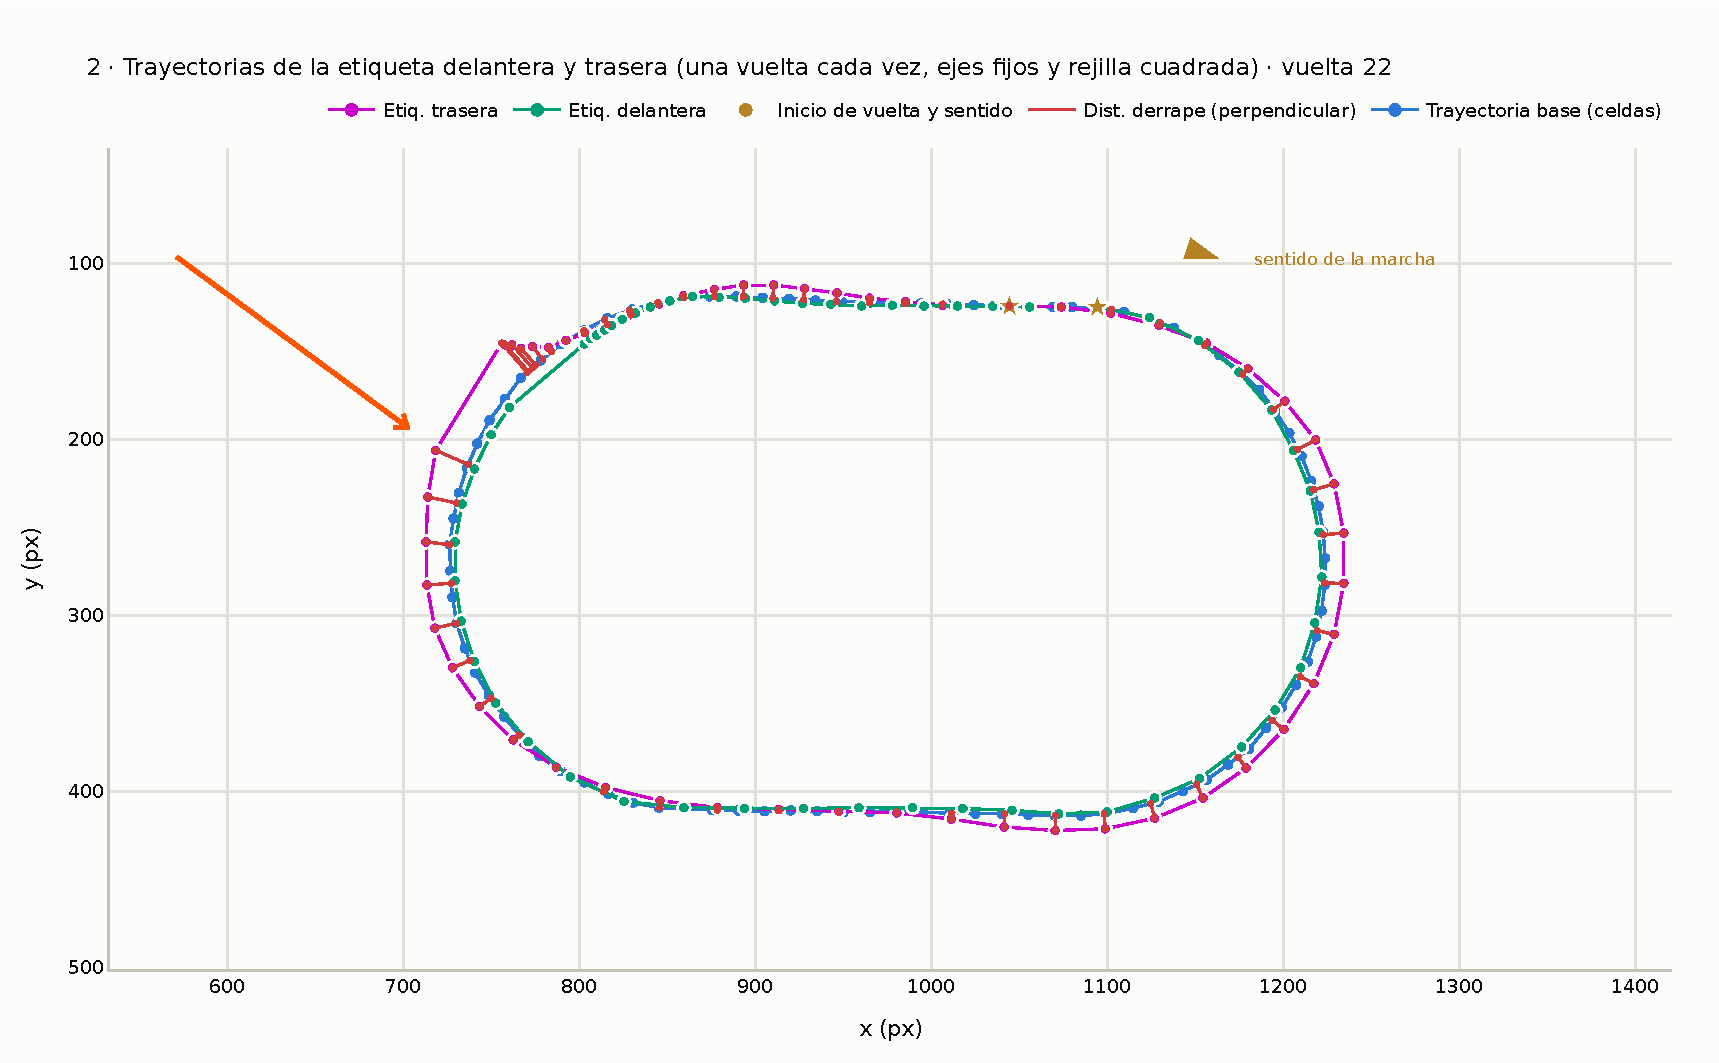
\includegraphics[trim={0 0 0 42pt},clip,width=\linewidth]{imaxes/PRUEBAS/COMPARATIVA_COCHES/dist_derrape_coche_azul.pdf}
    \caption{Coche azul}
    \label{fig:comparativa-trayectorias-azul}
  \end{subfigure}

  \vspace{1em}

  \begin{subfigure}[b]{\textwidth}
    \centering
    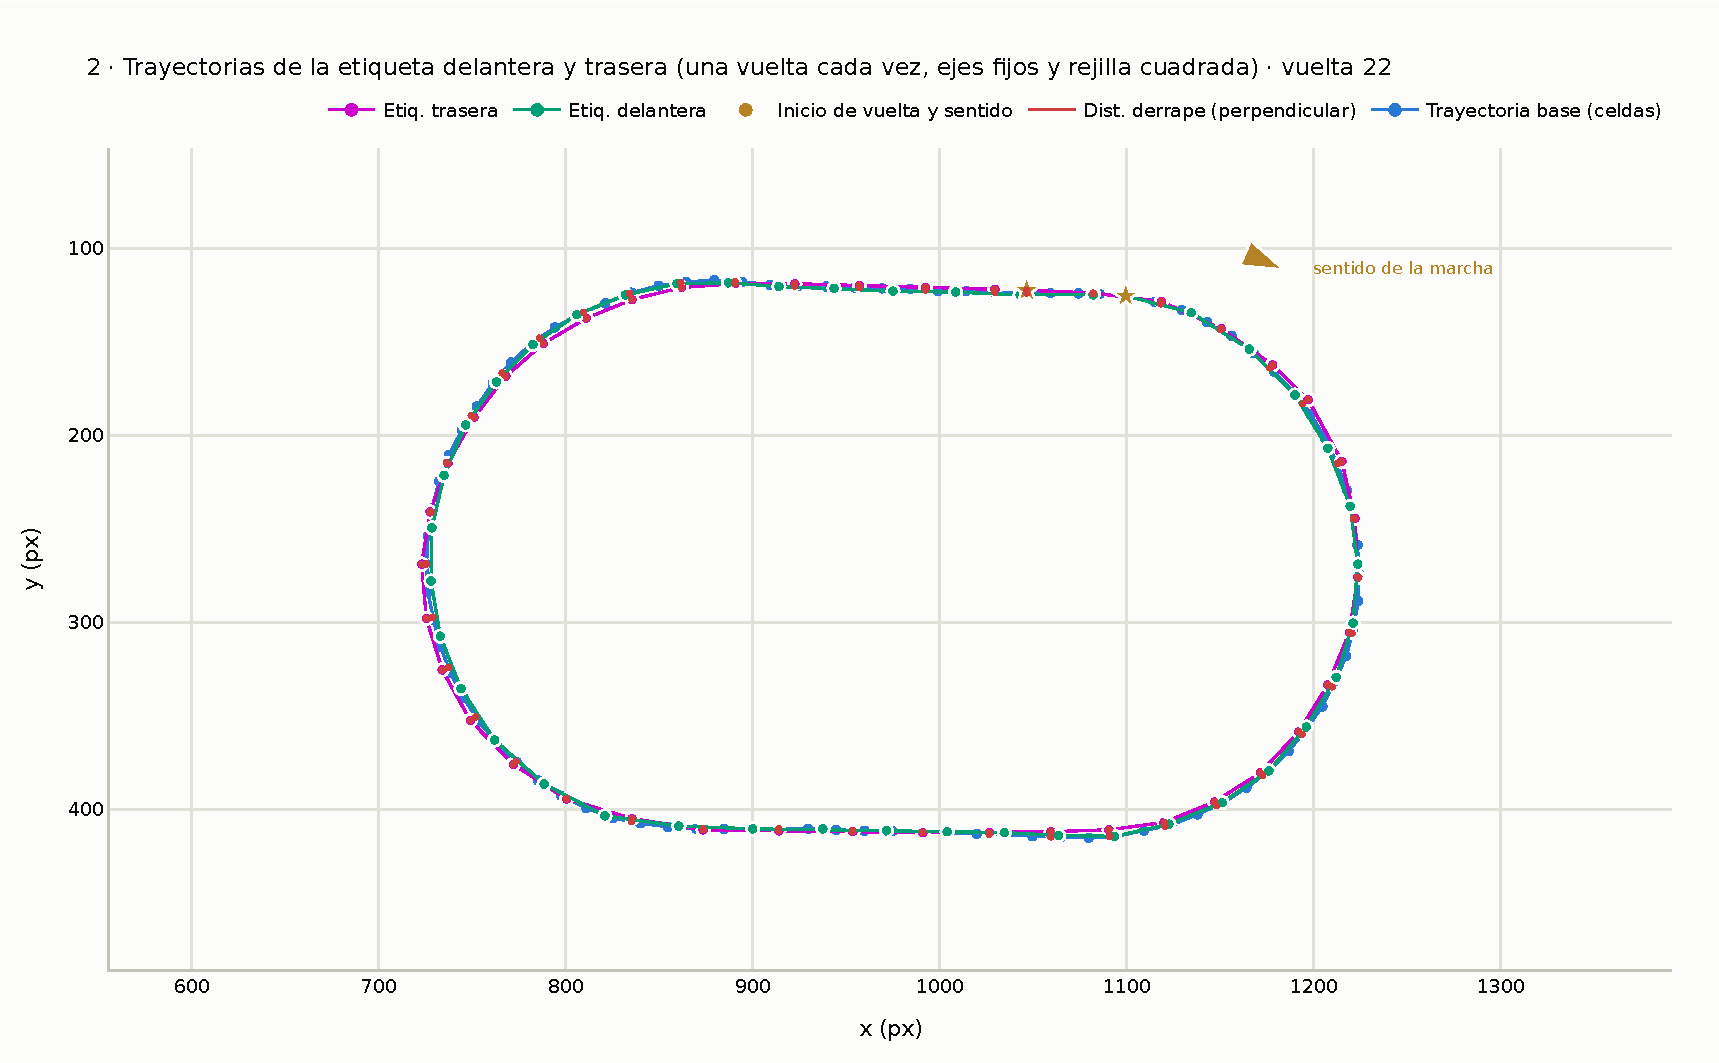
\includegraphics[trim={0 0 0 42pt},clip,width=\linewidth]{imaxes/PRUEBAS/COMPARATIVA_COCHES/dist_derrape_coche_rojo.pdf}
    \caption{Coche rojo}
    \label{fig:comparativa-trayectorias-rojo}
  \end{subfigure}
  \caption{Trayectoria de las dos etiquetas en la vuelta 22 con la misma configuración del algoritmo.}
  \label{fig:comparativa-trayectorias}
\end{figure}

Una vez detectado el derrape el algoritmo castiga al coche azul y genera dos zonas, como se aprecia en la figura~\ref{fig:comparativa-zonas-azul}, la zona de derrape, que cubre las celdas 47 a 68 y queda limitada a PWM 89, y la que ya venía de antes, que se mantiene en 91. En el coche rojo no hubo ningún derrape que castigar y por tanto no se abre ninguna zona nueva, de modo que en la figura~\ref{fig:comparativa-zonas-rojo} sigue habiendo una única zona que además ha continuado subiendo hasta PWM 92.

\begin{figure}[tbp]
  \centering
  \begin{subfigure}[b]{\textwidth}
    \centering
    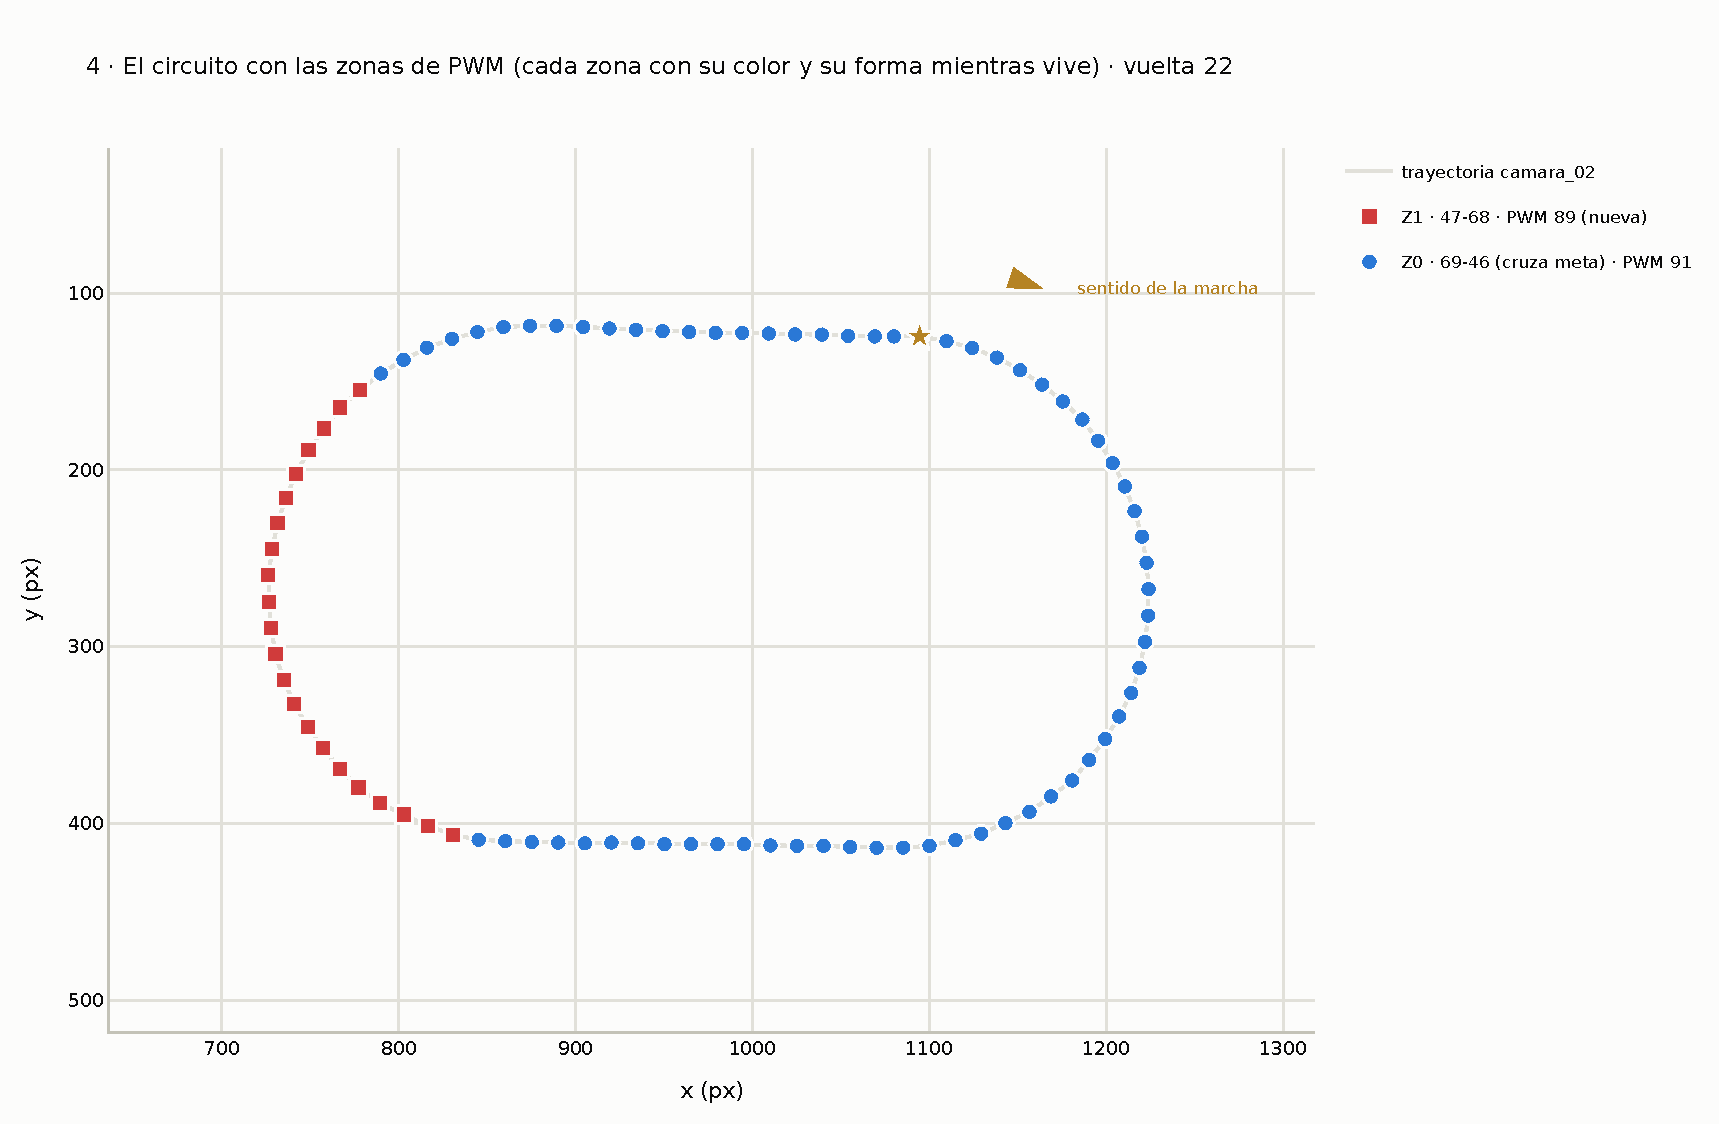
\includegraphics[trim={0 0 0 60pt},clip,page=1,width=\linewidth]{imaxes/PRUEBAS/COMPARATIVA_COCHES/pwm_zonas_coche_azul.pdf}
    \caption{Coche azul}
    \label{fig:comparativa-zonas-azul}
  \end{subfigure}

  \vspace{1em}

  \begin{subfigure}[b]{\textwidth}
    \centering
    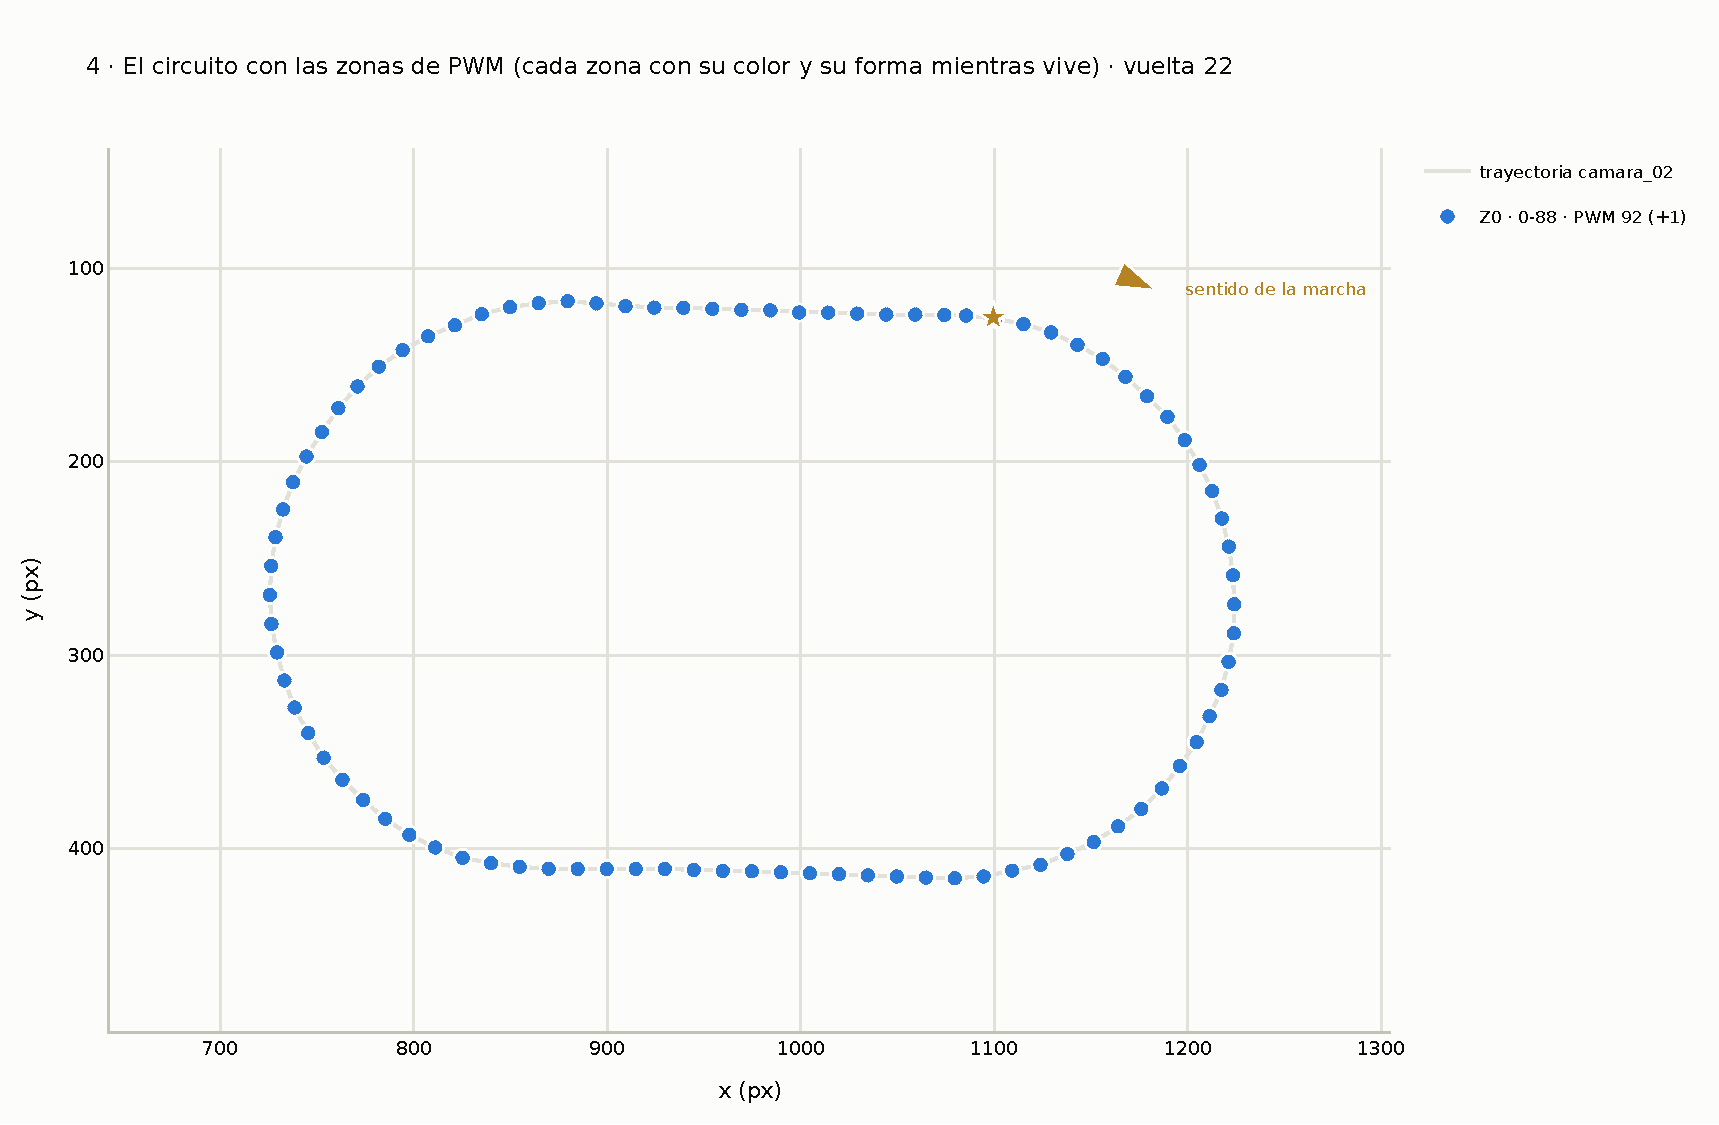
\includegraphics[trim={0 0 0 60pt},clip,page=1,width=\linewidth]{imaxes/PRUEBAS/COMPARATIVA_COCHES/pwm_zonas_coche_rojo.pdf}
    \caption{Coche rojo}
    \label{fig:comparativa-zonas-rojo}
  \end{subfigure}
  \caption{Partición del circuito en zonas de PWM en la vuelta 22. El coche azul arrastra una zona de derrape ya castigada y el rojo mantiene una única zona libre que sigue subiendo.}
  \label{fig:comparativa-zonas}
\end{figure}

El comportamiento no es puntual, sino que se repite a lo largo de toda la ejecución, como recoge la figura~\ref{fig:comparativa-derrapes}, donde se representa vuelta a vuelta la distancia de derrape registrada junto al PWM medio aplicado. El coche azul encadena picos muy por encima del umbral, varios de ellos por encima de los 20~px, que se corresponden con derrapes lo bastante fuertes como para que el coche estuviera a punto de salirse de la pista. En el coche rojo los máximos se mantienen entre los 4 y los 9~px durante toda la carrera y ninguno llega a superar el umbral.

\begin{figure}[tbp]
  \centering
  \begin{subfigure}[b]{\textwidth}
    \centering
    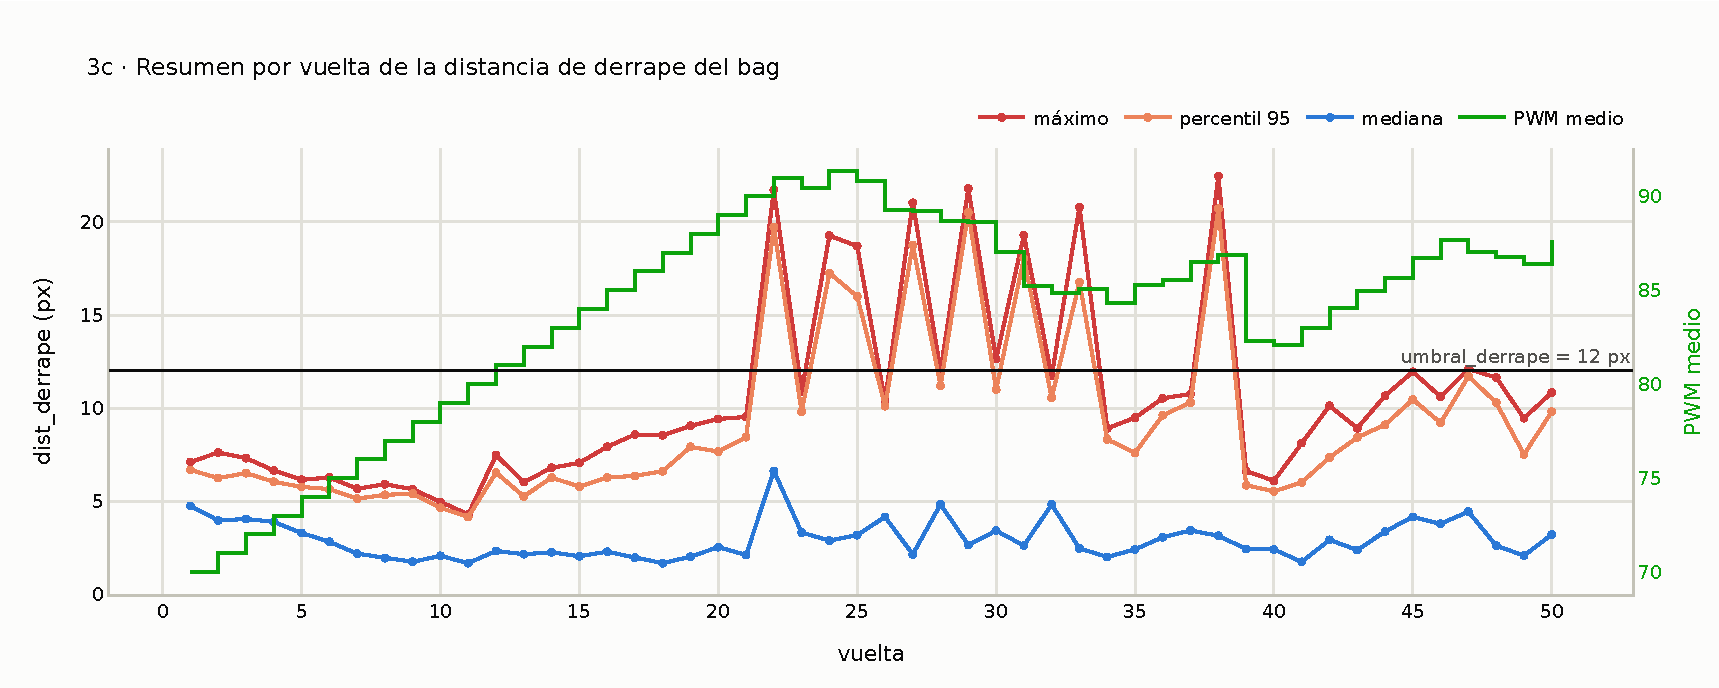
\includegraphics[trim={0 0 0 44pt},clip,width=\linewidth]{imaxes/PRUEBAS/COMPARATIVA_COCHES/resumen_derrapes_coche_azul.pdf}
    \caption{Coche azul}
    \label{fig:comparativa-derrapes-azul}
  \end{subfigure}

  \vspace{1em}

  \begin{subfigure}[b]{\textwidth}
    \centering
    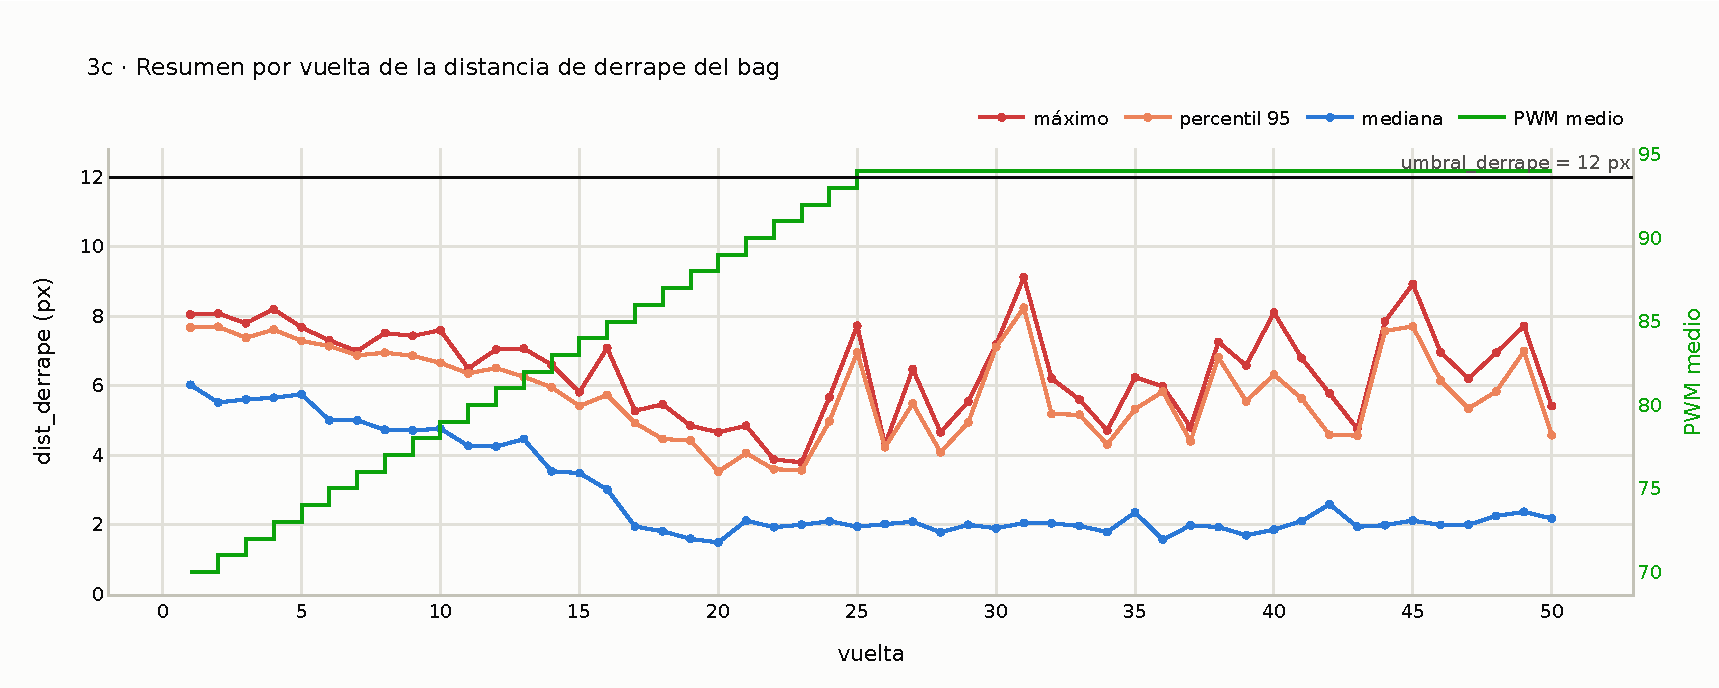
\includegraphics[trim={0 0 0 44pt},clip,width=\linewidth]{imaxes/PRUEBAS/COMPARATIVA_COCHES/resumen_derrapes_coche_rojo.pdf}
    \caption{Coche rojo}
    \label{fig:comparativa-derrapes-rojo}
  \end{subfigure}
  \caption{Resumen por vuelta de cómo varió la distancia de derrape frente al PWM.}
  \label{fig:comparativa-derrapes}
\end{figure}

Los tiempos de las dos ejecuciones, recogidos en la tabla~\ref{tab:comparativa-coches}, confirman lo que muestran las gráficas. El coche rojo tarda 75,44~s en completar las 50 vueltas frente a los 93,59~s del azul, una diferencia de 18~segundos que supone más de un 19\,\% del tiempo total con el mismo algoritmo y la misma configuración. El origen no está en el control, sino en el propio coche, que pierde adherencia con valores de PWM que el rojo asimila sin problema.

\begin{table}[tbp]
  \centering
  \estilotabla[3]
  \caption{Métricas de tiempo por vuelta de ambos coches con la misma configuración (PWM 70--94, umbral de derrape 12~px).}
  \label{tab:comparativa-coches}
  \begin{tabular}{lrrrrr}
    \toprule
    \rowcolor{ArqAzulClaro}
    Coche & Contrarreloj & Mejor & Mediana & Media & $\sigma$ \\
          \rowcolor{ArqAzulClaro} & (s) & (s) & (s) & (s) & (s) \\
    \midrule
    Azul & 93,59 & 1,661 & 1,755 & 1,872 & 0,228 \\
    Rojo & 75,44 & 1,315 & 1,377 & 1,509 & 0,232 \\
    \bottomrule
  \end{tabular}
\end{table}

El problema no afecta solo al algoritmo, porque en las pruebas de conducción manual de la sección~\ref{sec:prueba-algo-vs-personas} a las personas también les cuesta más controlar el coche azul, ya que es mucho más sensible a los valores altos de PWM. La consecuencia práctica de todo esto es que no existe una configuración única válida para los dos coches y que los parámetros del algoritmo, en particular el umbral de derrape, deben ajustarse a las características del vehículo, que es lo que se comprueba en la prueba~\ref{sec:prueba-algo-parametros}.

\section{Prueba PWM incremental}
\label{sec:prueba_pwm_incremental}

Durante las pruebas unitarias aparecieron problemas en el comportamiento del circuito, los valores y las configuraciones que servían un día para un coche ya no eran valían al día siguiente. Igual que en la prueba anterior, todos los nodos se lanzaron en un mismo ordenador para que la red no influyera en el control del coche, y para ver el comportamiento para un PWM se aplico el modo incremental, descrito en la sección~\ref{subsec:modos-operacion}, aumentado el valor cada 10 vueltas. Se realizaron seis ejecuciones que recogidas en la tabla~\ref{tab:incremental-sesiones}, se usaron los dos coches y en dos días distintos.

\begin{table}[tbp]
  \centering
  \estilotabla[3]
  \caption{Resumen ejecuciones de la prueba con PWM incremental.}
  \label{tab:incremental-sesiones}
  \begin{tabular}{llcrcrc}
    \toprule
    \rowcolor{ArqAzulClaro}
    Coche & Día & Sesión & Vueltas & PWM & Mejor & Sin mejora \\
          \rowcolor{ArqAzulClaro} & & & & & (s) & desde PWM \\
    \midrule
    Azul & 22/07 & 001 & 243 & 70--93  & 1,697 & 74 \\
    Azul & 22/07 & 002 & 236 & 70--92  & 1,702 & 85 \\
    Azul & 03/09 & ---  & 361 & 75--110 & 1,863 & 92 \\
    Rojo & 22/07 & 001 & 277 & 70--95  & 1,581 & 93 \\
    Rojo & 22/07 & 002 & 261 & 70--95  & 1,584 & 93 \\
    Rojo & 03/09 & ---  & 360 & 75--110 & 1,350 & 98 \\
    \bottomrule
  \end{tabular}
\end{table}

Con el coche azul, el 22/07 una vuelta se daba en 1,774~s con un PWM de 75, mientras que el 03/09 ese mismo valor necesitaba 3,095~s y hubo que llegar hasta 110 para acercarse al tiempo que el otro día se conseguía con 74. Con el coche rojo ocurre justo lo contrario, porque el 03/09 fue más rápido que el 22/07 en todos los valores comunes, entre 0,15 y 0,53~s por vuelta. Los números están en la tabla~\ref{tab:incremental-por-pwm}. Destacar que la distancia de derrape se mantiene en valores parecidos entre las sesiones, alrededor de 5~px el azul y de 9~px el rojo. 

\begin{table}[tbp]
  \centering
  \estilotabla[3]
  \caption{Tiempo por vuelta ($t$, mediana del escalón) y distancia de derrape ($d$, percentil 95) en los valores de PWM comunes a los dos días. Se usan las sesiones 001 del 22/07.}
  \label{tab:incremental-por-pwm}
  \begin{tabular}{lrrrrrrrr}
    \toprule
    \rowcolor{ArqAzulClaro}
    & \multicolumn{2}{c}{Azul 22/07} & \multicolumn{2}{c}{Azul 03/09}
    & \multicolumn{2}{c}{Rojo 22/07} & \multicolumn{2}{c}{Rojo 03/09} \\
    \rowcolor{ArqAzulClaro}
    PWM & $t$ (s) & $d$ (px) & $t$ (s) & $d$ (px)
        & $t$ (s) & $d$ (px) & $t$ (s) & $d$ (px) \\
    \midrule
    75 & 1,774 & 4,9 & 3,095 & 5,7 & 2,351 & 8,8 & 1,825 & 10,8 \\
    80 & 1,781 & 5,1 & 2,457 & 5,1 & 2,167 & 8,2 & 1,596 & 9,8 \\
    85 & 1,774 & 5,7 & 2,226 & 4,4 & 1,911 & 8,0 & 1,515 & 9,2 \\
    90 & 1,763 & 6,1 & 2,029 & 5,2 & 1,737 & 7,1 & 1,510 & 9,1 \\
    93 & 1,767 & 6,2 & 1,954 & 6,2 & 1,633 & 6,6 & 1,480 & 8,7 \\
    \bottomrule
  \end{tabular}
\end{table}

Apartir de los resultados obtenidos tambin se aprecia que pasado cierto punto subir el PWM deja de mejorar el tiempo. La figura~\ref{fig:incremental-escalera} lo enseña el coche azul del 22/07 baja de 2,00 a 1,78~s entre los valores 70 y 74, y ahí se queda clavado, de manera que los diecinueve escalones que vienen después, hasta el 93, no tienen gran impacto en el tiempo. El del 03/09 sigue mejorando un poco más, hasta el 92, y a partir de ahí se estanca igual. El problema, por tanto, no es solo que haya que aplicar un PWM mayor, sino que ni aplicándolo se recuperan los tiempos de otros dias. Y al forzar el valor por arriba es cuando el coche acaba saliéndose, ya que el último escalón del 03/09 es el único de toda la prueba en el que el azul llega a descontrolarse, con vueltas de 2,8~s y separaciones de la trayectoria de hasta 37~px.

\begin{figure}[tbp]
  \centering
  \begin{subfigure}[b]{0.85\textwidth}
    \centering
    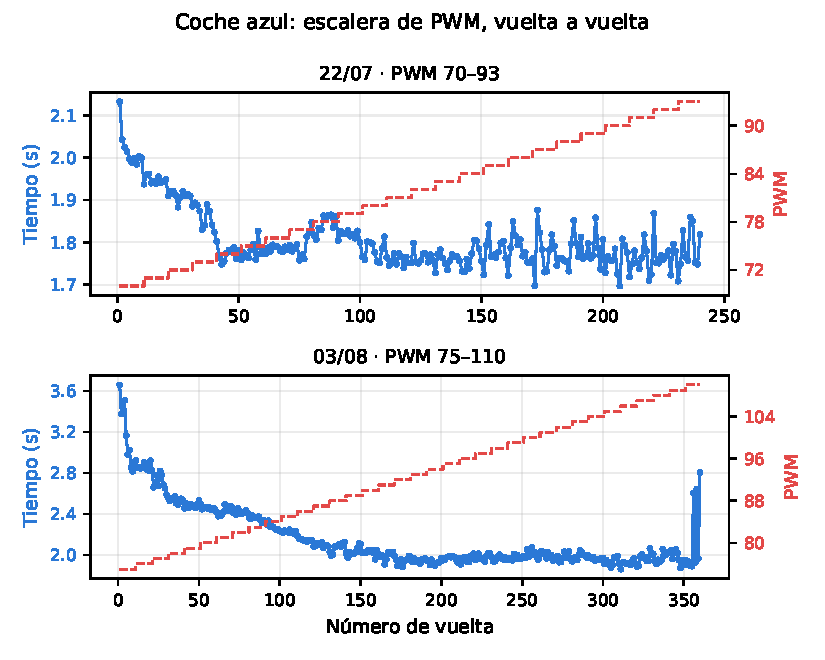
\includegraphics[trim={0 0 0 24},clip,width=\linewidth]{imaxes/PRUEBAS/PWM_INCREMENTAL/escalera_azul.pdf}
    \caption{Coche azul}
    \label{fig:incremental-escalera-azul}
  \end{subfigure}

  \vspace{0.5em}

  \begin{subfigure}[b]{0.85\textwidth}
    \centering
    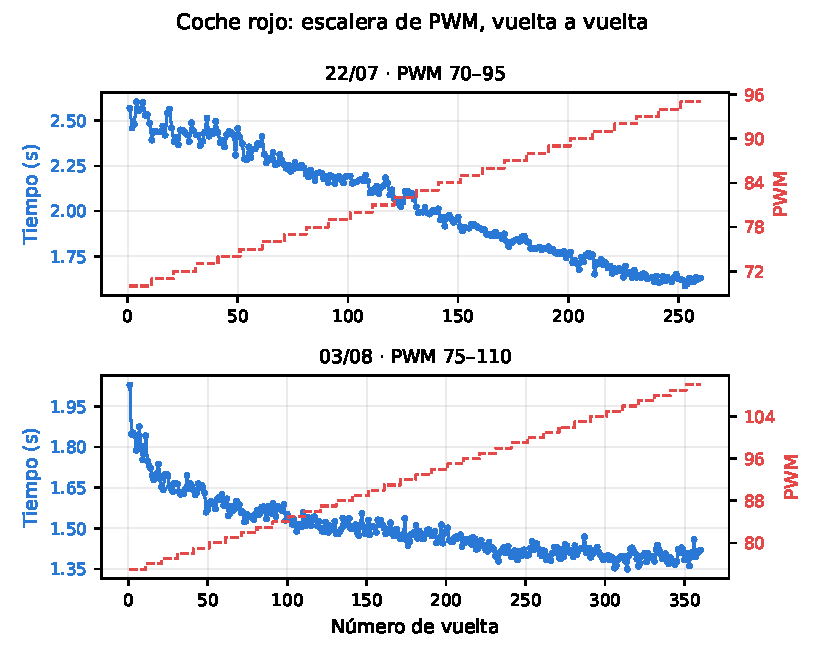
\includegraphics[trim={0 0 0 24},clip,width=\linewidth]{imaxes/PRUEBAS/PWM_INCREMENTAL/escalera_rojo.pdf}
    \caption{Coche rojo}
    \label{fig:incremental-escalera-rojo}
  \end{subfigure}
  \caption{Tiempo por vuelta y escalera de PWM de las dos sesiones de cada coche.}
  \label{fig:incremental-escalera}
\end{figure}

La causa más probable de estos problemas sea el propio montaje de la pista, que exige un buen contacto entre los carriles y que además se monta con piezas mezcladas de varios modelos de Scalextric, de manera que el comportamiento del coche no siempre es el esperado y resulta difícil predecirlo de un día para otro. Esto obliga a tener cuidado al cargar una política ya fijada, porque puede funcionar un día y dejar de hacerlo en otro. Con el algoritmo el problema se puede sortear, ya que basta con relanzarlo o cambiar sus parámetros en caliente, pero no deja de ser un apaño y es una de las limitaciones que se le detectaron, porque no llega a adaptarse por sí solo al comportamiento del circuito. Un algoritmo suficientemente bueno subiría su propio techo de PWM al ver que el circuito no responde, y eso no se contempló durante el diseño porque no se esperaba este comportamiento, que en los trabajos anteriores no aparece reportado.

\section{Prueba de ajuste de los parámetros del algoritmo}
\label{sec:prueba-algo-parametros}

El parámetro sobre el que tiene sentido actuar es el umbral de derrape, que determina a partir de qué separación de la etiqueta trasera respecto a la trayectoria base se considera que el coche está derrapando. Se reprodujeron las mismas condiciones de la sección~\ref{sec:prueba-comparativa-coches}, con el circuito en óvalo cubierto por una sola cámara, todos los nodos en la misma máquina y 50 vueltas por ejecución, y se realizaron tres ejecuciones con el coche azul variando el techo de PWM y el umbral.

La figura~\ref{fig:parametros-tiempos} compara la evolución del tiempo por vuelta con los dos umbrales. Con 9~px el algoritmo detecta los derrapes antes de que empiecen a ser problemáticos (los que se producen cuando el coche empieza a coger velocidad y a ganar inercia), y baja la potencia del carril antes de que el derrape llegue a manifestarse, con lo que la curva se estabiliza a partir de la vuelta 12 y el peor tiempo queda en las primeras vueltas. Con 12~px aparecen entre las vueltas 21 y 38 los picos señalados en la gráfica, que se corresponden con derrapes como el de la figura~\ref{fig:comparativa-trayectorias-azul} y en los que el coche llega casi a salirse de la pista y necesita varias vueltas para recuperar el ritmo, de manera que se vuelve prácticamente a los tiempos que teníamos antes de empezar la carrera.

\begin{figure}[tbp]
  \centering
  \begin{subfigure}[b]{\textwidth}
    \centering
    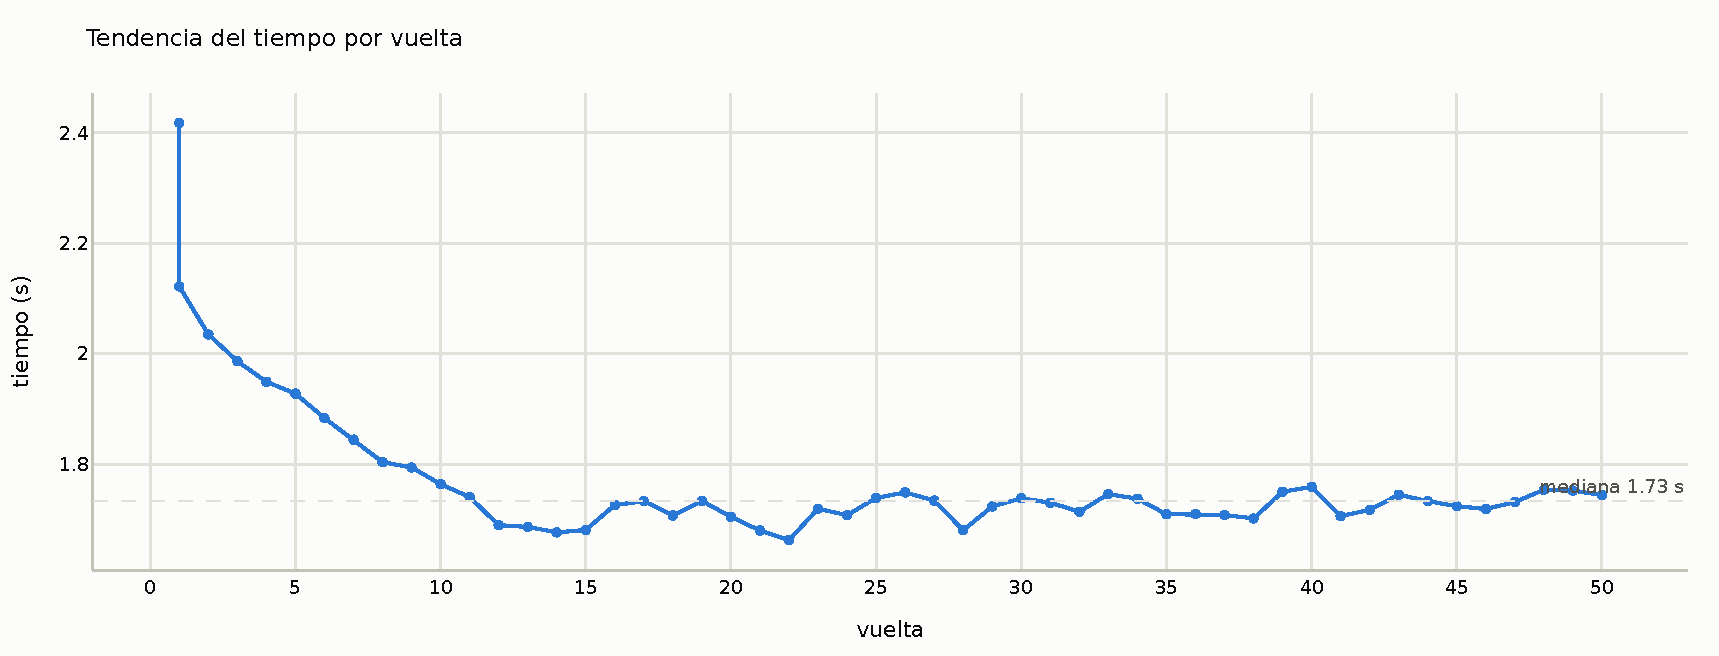
\includegraphics[trim={0 0 0 38pt},clip,width=\linewidth]{imaxes/PRUEBAS/ALGO_VARIOS_PARAMETROS/tiempos_vuelta_mejora_azul.pdf}
    \caption{Umbral de derrape 9~px}
    \label{fig:parametros-tiempos-mejor}
  \end{subfigure}

  \vspace{1em}

  \begin{subfigure}[b]{\textwidth}
    \centering
    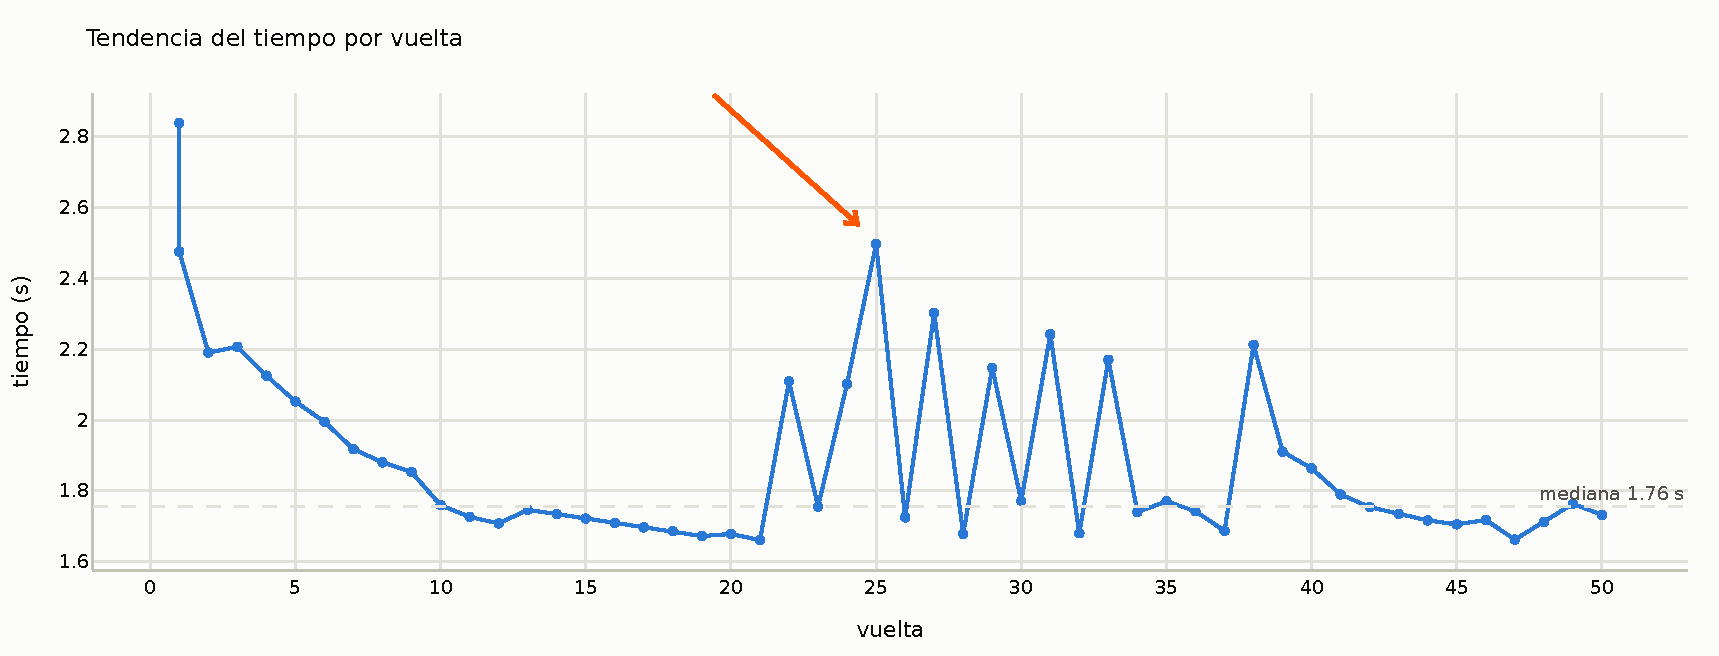
\includegraphics[trim={0 0 0 38pt},clip,width=\linewidth]{imaxes/PRUEBAS/ALGO_VARIOS_PARAMETROS/tiempos_vuelta_peor_azul.pdf}
    \caption{Umbral de derrape 12~px}
    \label{fig:parametros-tiempos-peor}
  \end{subfigure}
  \caption{Evolución del tiempo por vuelta del coche azul en el circuito en óvalo con PWM 70--94 y dos umbrales de derrape distintos.}
  \label{fig:parametros-tiempos}
\end{figure}

La razón de esos picos se ve en la figura~\ref{fig:parametros-derrapes}. Con el umbral en 9~px los derrapes siguen produciéndose, pero se mantienen acotados alrededor de esa misma cifra y solo en unas pocas vueltas llegan a los 10~px, mientras que con el umbral en 12~px el sistema no reacciona hasta que el derrape ya está desarrollado y para entonces el castigo llega tarde, con máximos que se disparan por encima de los 20~px. Ese contraste se aprecia mejor en la figura~\ref{fig:derrape-vuelta}. Con el umbral en 9~px el derrape se detecta mientras todavía está creciendo y el pico se queda en los 10~px, mientras que con 12~px se produce un salto de esa misma franja hasta los 19~px sin ningún paso intermedio. La nube de puntos grises del fondo, que acumula todas las vueltas de la ejecución, se concentra justo entre los 9 y los 10~px, de manera que ahí está la frontera y una vez superada el derrape ya no se puede contener.

\begin{figure}[tbp]
  \centering
  \begin{subfigure}[b]{\textwidth}
    \centering
    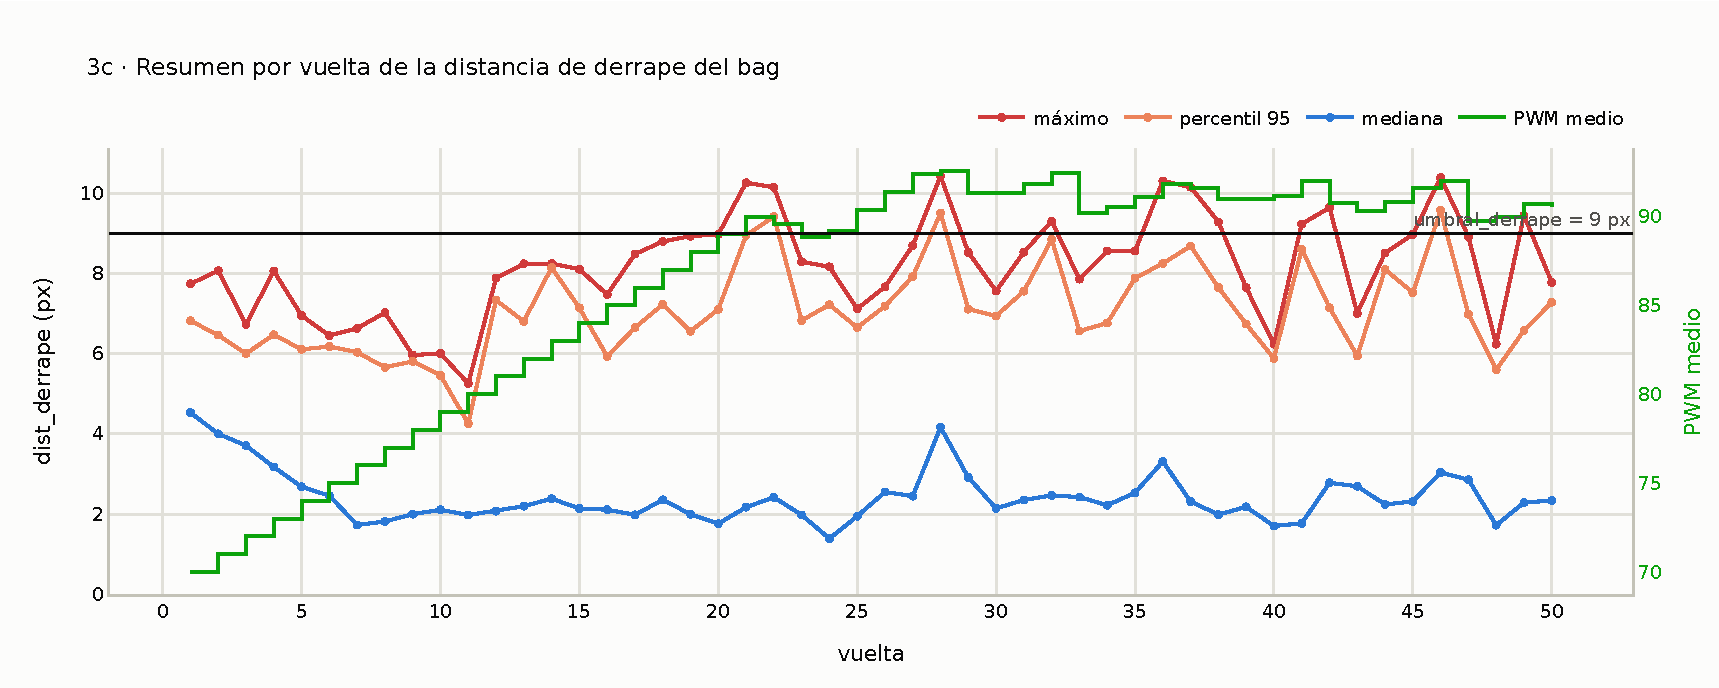
\includegraphics[trim={0 0 0 44pt},clip,width=\linewidth]{imaxes/PRUEBAS/ALGO_VARIOS_PARAMETROS/resumen_dist_derrapes_mejora_azul.pdf}
    \caption{Umbral de derrape 9~px}
    \label{fig:parametros-derrapes-mejor}
  \end{subfigure}

  \vspace{1em}

  \begin{subfigure}[b]{\textwidth}
    \centering
    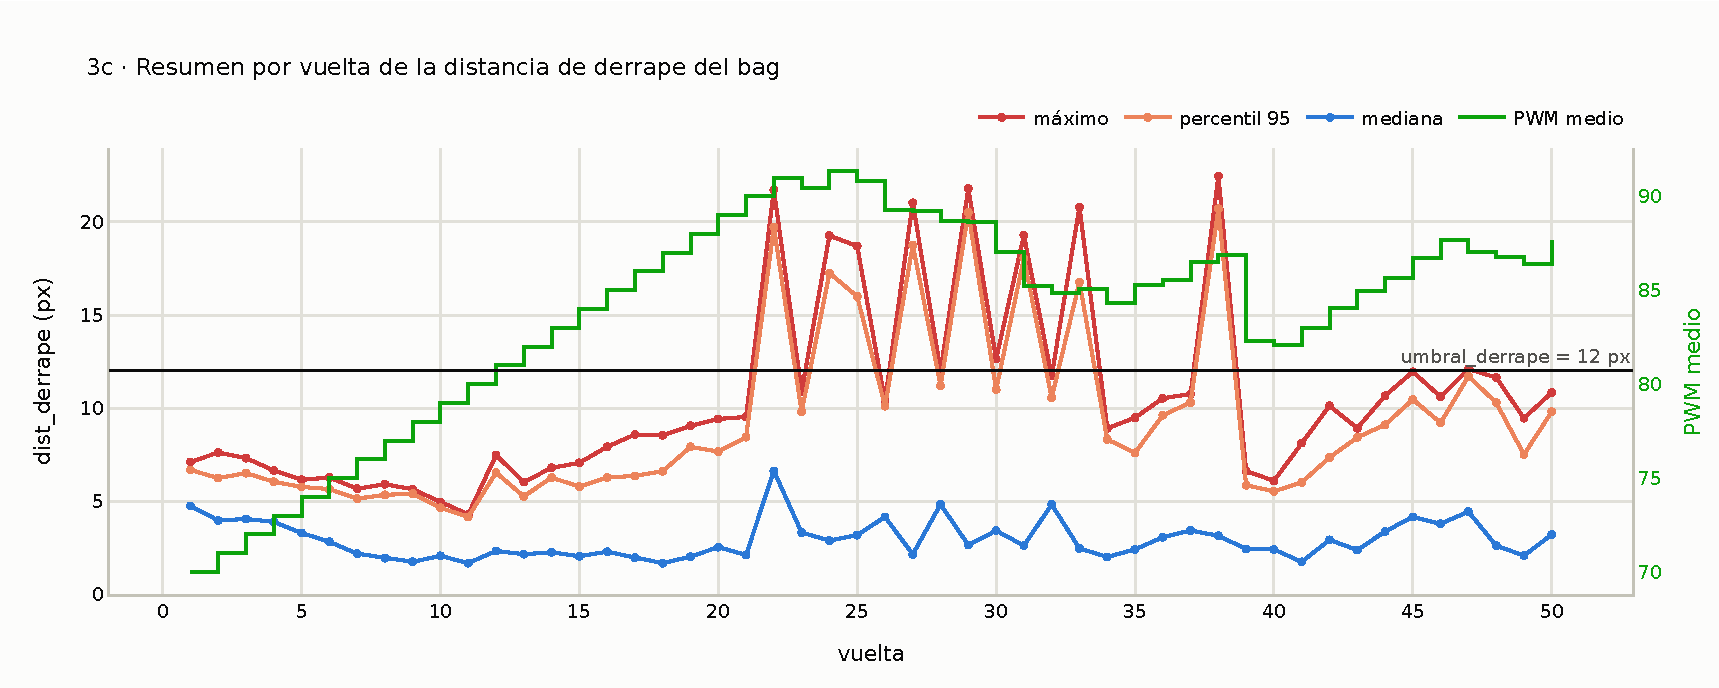
\includegraphics[trim={0 0 0 44pt},clip,width=\linewidth]{imaxes/PRUEBAS/ALGO_VARIOS_PARAMETROS/resumen_dist_derrapes_peor_azul.pdf}
    \caption{Umbral de derrape 12~px}
    \label{fig:parametros-derrapes-peor}
  \end{subfigure}
  \caption{Resumen por vuelta de la distancia de derrape del coche azul con los dos umbrales.}
  \label{fig:parametros-derrapes}
\end{figure}

\begin{figure}[tbp]
  \centering
  \begin{subfigure}[b]{\textwidth}
    \centering
    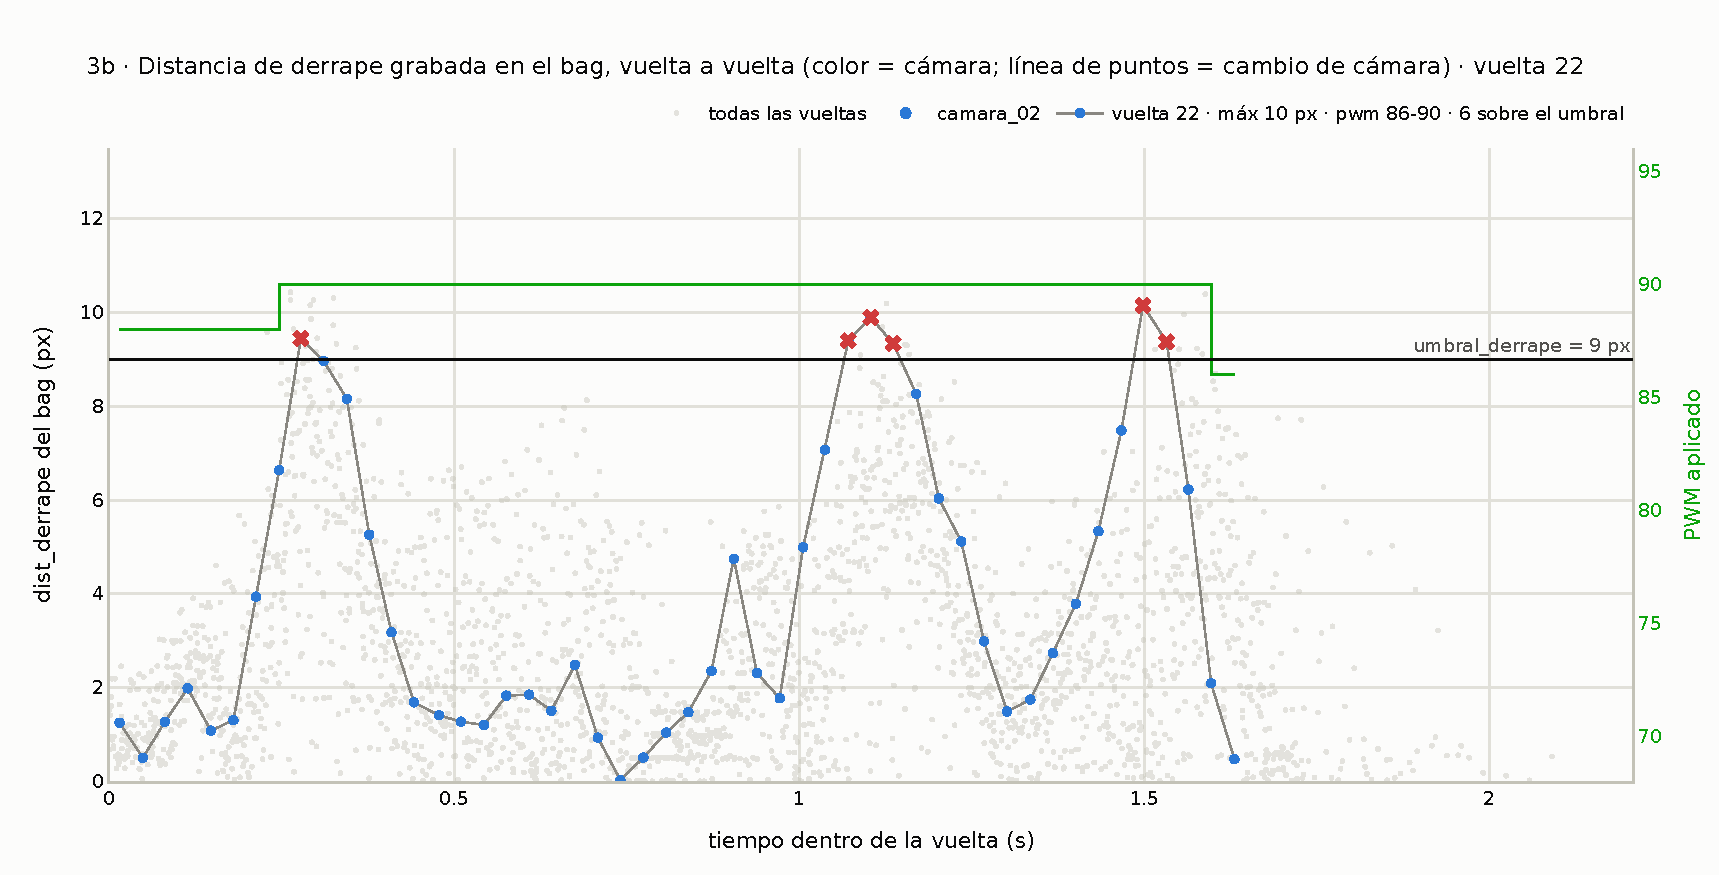
\includegraphics[trim={0 0 0 43pt},clip,width=\linewidth]{imaxes/PRUEBAS/ALGO_VARIOS_PARAMETROS/derrape_controlado.pdf}
    \caption{Umbral de derrape 9~px, vuelta 22}
    \label{fig:derrape-controlado}
  \end{subfigure}

  \vspace{1em}

  \begin{subfigure}[b]{\textwidth}
    \centering
    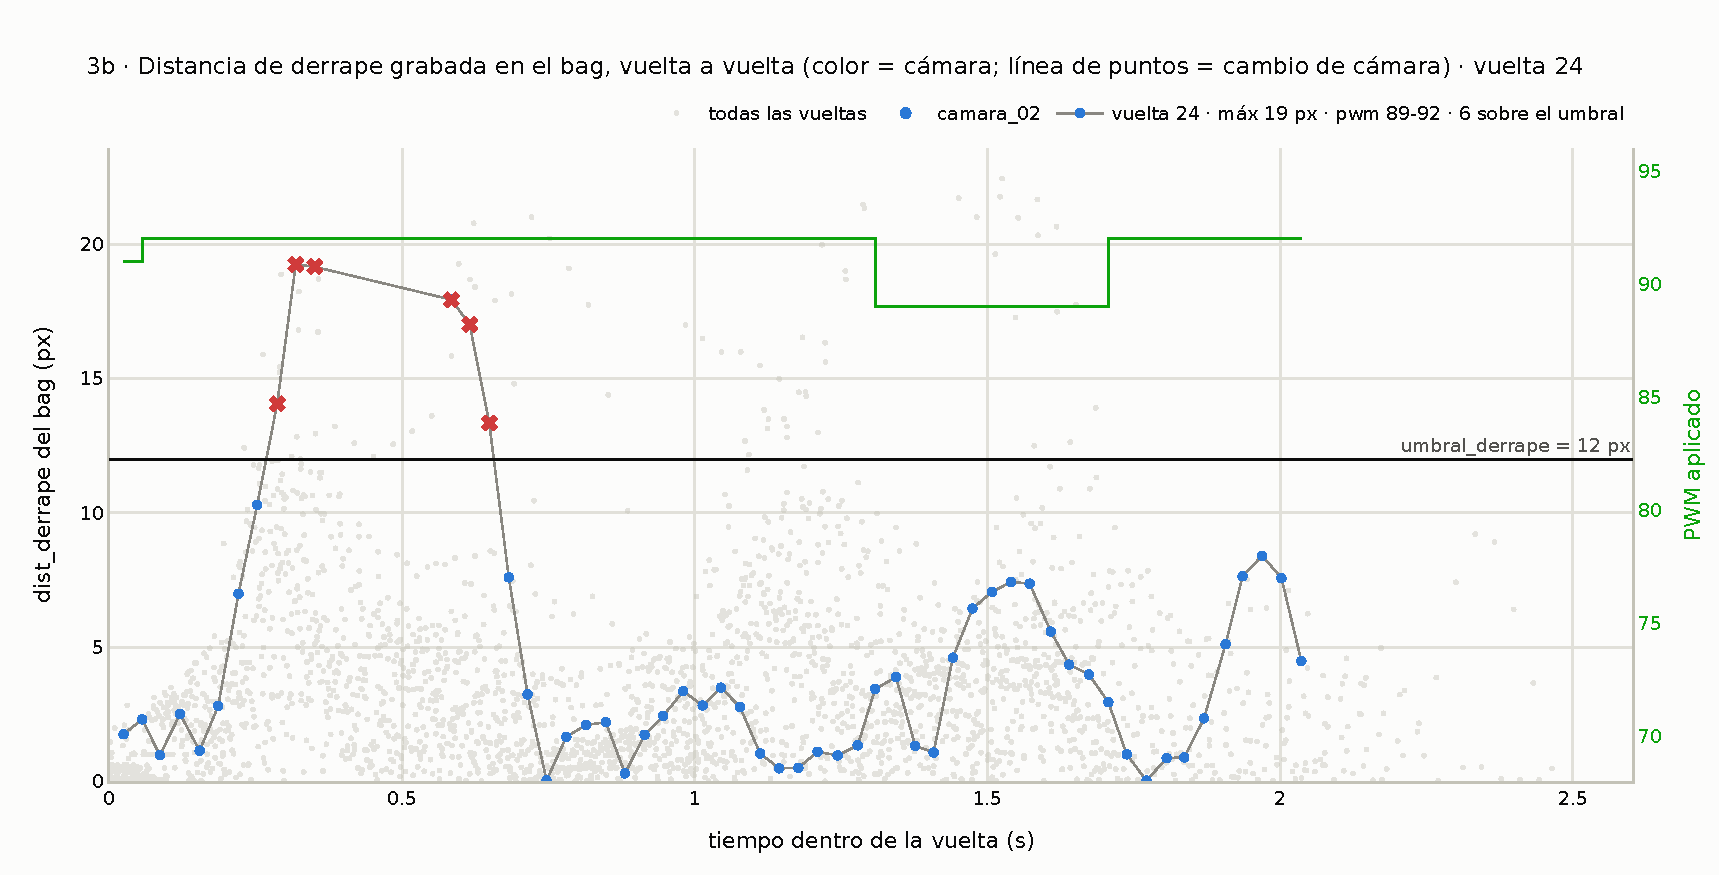
\includegraphics[trim={0 0 0 43pt},clip,width=\linewidth]{imaxes/PRUEBAS/ALGO_VARIOS_PARAMETROS/derrape_explosivo.pdf}
    \caption{Umbral de derrape 12~px, vuelta 24}
    \label{fig:derrape-explosivo}
  \end{subfigure}
  \caption{Saltos en la distancia de derrape del coche azul. Las cruces rojas son las muestras que superan el umbral y el fondo gris, el resto de vueltas de la ejecución}
  \label{fig:derrape-vuelta}
\end{figure}

Las métricas de las tres ejecuciones se recogen en la tabla~\ref{tab:parametros-azul} y permiten precisar en qué consiste la mejora. Las medianas de las dos configuraciones con PWM 70--94 son casi iguales, 1,733~s frente a 1,755~s, y las mejores vueltas resultan indistinguibles, 1,663~s frente a 1,661~s, de modo que bajar el umbral no hace al coche más rápido en su vuelta buena, sino que le quita las vueltas malas. Eso se refleja en la media, que cae de 1,872~s a 1,759~s, y en la peor vuelta, que pasa de 2,839~s a 2,418~s, y sobre todo en la desviación típica, que se reduce a menos de la mitad, de 0,228~s a 0,094~s. Sobre las 50 vueltas la diferencia acumulada es de 5,66~segundos, así que en una carrera entre ambas configuraciones ganaría la más conservadora, que mantiene el ritmo, frente a la que pierde varias décimas cada vez que tarda en detectar un derrape.

\begin{table}[tbp]
  \centering
  \estilotabla[3]
  \caption{Métricas de tiempo por vuelta del coche azul en el circuito en óvalo para las tres configuraciones probadas.}
  \label{tab:parametros-azul}
  \begin{tabular}{lrrrrr}
    \toprule
    \rowcolor{ArqAzulClaro}
    Ejecución & Contrarreloj & Mejor & Mediana & Media & $\sigma$ \\
              \rowcolor{ArqAzulClaro} & (s) & (s) & (s) & (s) & (s) \\
    \midrule
    ALGO 012 (70--90, 12~px) & 96,41 & 1,731 & 1,788 & 1,928 & 0,291 \\
    ALGO 013 (70--94, 12~px) & 93,59 & 1,661 & 1,755 & 1,872 & 0,228 \\
    ALGO 014 (70--94, 9~px)  & 87,93 & 1,663 & 1,733 & 1,759 & 0,094 \\
    \bottomrule
  \end{tabular}
\end{table}

ALGO 012 mantiene el umbral permisivo de 12~px pero rebaja el techo de PWM de 94 a 90, y es la peor de las tres en todas las métricas, con 96,41~s de tiempo acumulado y una desviación típica de 0,291~s. Bajar el techo de velocidad penaliza el ritmo sin resolver los derrapes, porque el problema no era ir demasiado deprisa sino reaccionar demasiado tarde, y por eso la mejora viene de afinar el umbral y no de conducir más despacio.

\section{Prueba del algoritmo frente a pilotos humanos}
\label{sec:prueba-algo-vs-personas}

Existe una prueba equivalente en el trabajo de Adrián~\cite{tfgadrian}, pero abarca muy pocas vueltas y no es lo suficientemente preciso en el análisis.

Para las ejecuciones automáticas se reutilizaron los datos de las pruebas de las secciones~\ref{sec:prueba-comparativa-coches} y~\ref{sec:prueba-algo-parametros}. Para las manuales se levantó un nodo de cámara y un nodo controlador en la misma máquina, con el controlador en modo manual, se detalla cómo funciona en la sección~\ref{subsec:modos-operacion}. Cada piloto completó también 50 vueltas y después se apagó el sistema, con lo que todas las ejecuciones son directamente comparables.

La prueba se repitió en dos circuitos. El primero es el óvalo ya empleado en las pruebas anteriores, cubierto por una sola cámara. El segundo es el circuito en ocho, que necesita dos cámaras, una de ellas en la misma máquina que el nodo controlador y el puente Arduino y la otra en un segundo equipo que envía sus detecciones por red, de modo que este escenario añade la conmutación entre cámaras y la latencia de la red.

Las tablas~\ref{tab:vs-personas-azul} y~\ref{tab:vs-personas-rojo} recogen los resultados sobre el óvalo y en los dos coches se repite el mismo patrón. Los pilotos humanos firman las mejores vueltas absolutas, 1,276~s y 1,291~s en el coche rojo frente a los 1,315~s de la mejor ejecución automática, pero ninguno de los dos gana la contrarreloj. La explicación está en la desviación típica, de 0,787~s y 1,151~s en el caso de los pilotos frente a valores en torno a 0,22~s en las ejecuciones automáticas. El piloto encuentra el límite del coche en una vuelta concreta y no consigue repetirlo, y cada intento fallido le cuesta más de lo que le había ganado el intento bueno.

\begin{table}[tbp]
  \centering
  \estilotabla[3]
  \caption{Coche azul en el circuito en óvalo, algoritmo vs pilotos humanos.}
  \label{tab:vs-personas-azul}
  \begin{tabular}{lrrrrr}
    \toprule
    \rowcolor{ArqAzulClaro}
    Ejecución & Contrarreloj & Mejor & Mediana & Media & $\sigma$ \\
              \rowcolor{ArqAzulClaro} & (s) & (s) & (s) & (s) & (s) \\
    \midrule
    ALGO 014 (70--94, 9~px)  & 87,93 & 1,663 & 1,733 & 1,759 & 0,094 \\
    ALGO 013 (70--94, 12~px) & 93,59 & 1,661 & 1,755 & 1,872 & 0,228 \\
    Manual (piloto 1)        & 94,30 & 1,659 & 1,833 & 1,886 & 0,197 \\
    ALGO 012 (70--90, 12~px) & 96,41 & 1,731 & 1,788 & 1,928 & 0,291 \\
    Manual (piloto 2)        & 107,54 & 1,674 & 1,911 & 2,151 & 0,646 \\
    \bottomrule
  \end{tabular}
\end{table}

\begin{table}[tbp]
  \centering
  \estilotabla[3]
  \caption{Coche rojo en el circuito en óvalo, algoritmo vs pilotos humanos.}
  \label{tab:vs-personas-rojo}
  \begin{tabular}{lrrrrr}
    \toprule
    \rowcolor{ArqAzulClaro}
    Ejecución & Contrarreloj & Mejor & Mediana & Media & $\sigma$ \\
              \rowcolor{ArqAzulClaro} & (s) & (s) & (s) & (s) & (s) \\
    \midrule
    ALGO 013 (70--94, 12~px) & 75,44 & 1,315 & 1,377 & 1,509 & 0,232 \\
    ALGO 014 (70--94, 9~px)  & 75,67 & 1,329 & 1,399 & 1,513 & 0,214 \\
    ALGO 012 (70--90, 12~px) & 80,82 & 1,436 & 1,510 & 1,616 & 0,220 \\
    Manual (piloto 1)        & 82,36 & 1,291 & 1,421 & 1,647 & 0,787 \\
    Manual (piloto 2)        & 93,86 & 1,276 & 1,587 & 1,877 & 1,151 \\
    \bottomrule
  \end{tabular}
\end{table}

La diferencia entre los dos coches también reaparece aquí, como ya habíamos intuido en las pruebas anteriores. En el rojo la mejor ejecución automática le saca casi 7~segundos al mejor piloto, mientras que en el azul el margen se estrecha hasta los 0,7~segundos que separan a ALGO 013 del piloto 1, porque el coche es tan sensible que encontrar el punto de funcionamiento correcto resulta difícil para las dos partes. De hecho ALGO 012, con los parámetros mal ajustados, queda por debajo del piloto 1 en una de las ejecuciones.

% ---------------------------------------------------------------------
%  Circuito en ocho
% ---------------------------------------------------------------------

Los resultados sobre el circuito en ocho se recogen en las tablas~\ref{tab:vs-personas-ocho-azul} y~\ref{tab:vs-personas-ocho-rojo}. Este trazado es bastante más exigente que el óvalo, porque ya no basta con sostener una potencia constante: hay que frenar y volver a acelerar en los sitios adecuados.

\begin{table}[tbp]
  \centering
  \estilotabla[3]
  \caption{Coche azul en el circuito en ocho, algoritmo vs pilotos humanos.}
  \label{tab:vs-personas-ocho-azul}
  \begin{tabular}{lrrrrr}
    \toprule
    \rowcolor{ArqAzulClaro}
    Ejecución & Contrarreloj & Mejor & Mediana & Media & $\sigma$ \\
              \rowcolor{ArqAzulClaro} & (s) & (s) & (s) & (s) & (s) \\
    \midrule
    ALGO 002 (60--75, 9~px)  & 202,89 & 3,588 & 3,804 & 4,058 & 0,626 \\
    ALGO 004 (63--85, 8~px)  & 205,00 & 3,549 & 4,011 & 4,100 & 0,563 \\
    ALGO 001 (60--75, 10~px) & 210,22 & 3,576 & 3,885 & 4,204 & 0,733 \\
    ALGO 003 (60--85, 9~px)  & 243,92 & 3,697 & 4,200 & 4,878 & 2,094 \\
    Manual (piloto 2)        & 276,72 & 3,972 & 4,893 & 5,534 & 1,876 \\
    Manual (piloto 3)        & 427,23 & 4,615 & 6,589 & 8,545 & 4,997 \\
    \bottomrule
  \end{tabular}
\end{table}

En el coche azul la distancia entre el algoritmo y los pilotos se dispara respecto al óvalo. ALGO 002 completa las 50 vueltas en 202,89~s y el mejor de los dos pilotos necesita 276,72~s, un 36\,\% más, mientras que el segundo se va hasta los 427,23~s, más del doble. Aquí ya no se sostiene el consuelo del óvalo, porque la vuelta rápida también es del algoritmo, y ninguna de las cuatro configuraciones queda por detrás de un piloto, algo que allí sí llegó a pasar con ALGO 012. Entre esas cuatro se repite además el patrón de la sección~\ref{sec:prueba-algo-parametros}: ALGO 003 sube el techo de PWM a 85 sin tocar el umbral y es con diferencia la peor, con 243,92~s, mientras que ALGO 004 mantiene ese techo, baja el umbral a 8~px y vuelve a los 205,00~s, de modo que el techo se puede subir pero solo si el umbral se afina al mismo tiempo.

\begin{table}[tbp]
  \centering
  \estilotabla[3]
  \caption{Coche rojo en el circuito en ocho, algoritmo vs pilotos humanos.}
  \label{tab:vs-personas-ocho-rojo}
  \begin{tabular}{lrrrrr}
    \toprule
    \rowcolor{ArqAzulClaro}
    Ejecución & Contrarreloj & Mejor & Mediana & Media & $\sigma$ \\
              \rowcolor{ArqAzulClaro} & (s) & (s) & (s) & (s) & (s) \\
    \midrule
    ALGO 001 (60--75, 10~px)     & 138,23 & 2,603 & 2,713 & 2,765 & 0,152 \\
    Manual (piloto 1, intento 2) & 141,24 & 2,456 & 2,656 & 2,825 & 0,548 \\
    ALGO 003 (65--90, 10~px)     & 141,81 & 2,618 & 2,756 & 2,836 & 0,225 \\
    ALGO 002 (60--90, 10~px)     & 152,13 & 2,632 & 2,862 & 3,043 & 0,571 \\
    Manual (piloto 1, intento 4) & 154,87 & 2,387 & 2,567 & 3,097 & 1,307 \\
    Manual (piloto 1, intento 1) & 159,73 & 2,522 & 2,838 & 3,195 & 1,232 \\
    Manual (piloto 1, intento 3) & 162,10 & 2,424 & 2,689 & 3,242 & 1,659 \\
    Manual (piloto 2)            & 182,11 & 2,523 & 2,944 & 3,642 & 1,981 \\
    \bottomrule
  \end{tabular}
\end{table}

Con el coche rojo el resultado es mucho más ajustado, y es el que mejor ilustra la diferencia entre las dos formas de conducir. ALGO 001 gana la contrarreloj con 138,23~s y el mejor intento manual se queda a 3,01~s. El piloto 1 repitió la prueba cuatro veces y sus vueltas rápidas mejoraron en cada intento, de 2,522 a 2,387~s, hasta quedar por debajo de la mejor vuelta del algoritmo; en dos de ellos incluso su mediana, 2,656 y 2,567~s, baja de los 2,713~s de ALGO 001, así que su vuelta típica llega a ser más rápida que la del sistema. Lo que no mejora es el acumulado, porque sus cuatro contrarrelojes, 159,73, 141,24, 162,10 y 154,87~s, no dibujan ninguna tendencia.

La explicación está en las vueltas que la mediana no ve. Buscar la vuelta rápida saca el coche de la pista, y cada salida obliga a recogerlo, colocarlo y arrancar otra vez desde parado, de manera que un puñado de vueltas así borra todo lo ganado en las demás: la media ya se le da la vuelta al piloto, 2,825 y 3,097~s frente a los 2,765~s del algoritmo, y su desviación típica no baja de 0,548~s frente a los 0,152~s de ALGO 001. Si hubiese podido repetir su mejor vuelta las cincuenta veces habría cerrado en 119,35~s, casi 19~segundos por debajo del algoritmo, así que el margen existe; lo que no existe es la forma de sostenerlo. El piloto 2 es el mismo caso en su extremo, con una mejor vuelta perfectamente competitiva de 2,523~s y una contrarreloj de 182,11~s. Entre las configuraciones automáticas conviene señalar que ALGO 002 y ALGO 003 solo se diferencian en el suelo del rango, 60 frente a 65, y esos cinco puntos cuestan más de 10~segundos, 152,13 frente a 141,81~s: el suelo es el valor al que puede llegar el castigo, así que ajustar el rango no es solo cuestión de cuánto se deja correr al coche sino de cuánto se le permite frenar.

La comparación entre los dos coches vuelve a aparecer aquí y con más fuerza que en el óvalo. ALGO 001 se ejecutó con exactamente la misma configuración, con el rango de 60 a 75 y el umbral en 10~px, sobre los dos vehículos, y el resultado es de 210,22~s en el azul frente a 138,23~s en el rojo, casi 72~segundos y un 52\,\% más, cuando en el óvalo la misma comparación se quedaba en un 19\,\%. Un trazado más largo y con más curvas multiplica el efecto de la diferencia de adherencia descrita en la sección~\ref{sec:prueba-comparativa-coches}, y lo hace por igual para las dos partes, porque a los pilotos el coche azul también les cuesta mucho más que el rojo.

La conclusión de estas pruebas es que la ventaja del algoritmo no está en la velocidad punta sino en la capacidad de sostenerla. Un piloto humano iguala e incluso supera al sistema en una vuelta suelta, porque arriesga donde el algoritmo se limita a lo que ha aprendido, pero no consigue repetir ese riesgo cincuenta veces seguidas y en una carrera lo que cuenta es el acumulado. Cuanto más exigente es el trazado mayor es esa ventaja, porque la dificultad se le acumula al piloto vuelta tras vuelta mientras que al algoritmo solo le supone más zonas que ajustar. Esa regularidad es consecuencia directa de la política de castigo por zonas descrita en la sección~\ref{subsec:algoritmo-aprendizaje}, que sacrifica velocidad puntual en los tramos conflictivos a cambio de no perder vueltas enteras.

\section{Prueba de la política óptima}
\label{sec:prueba-politica-optima}

En esta prueba se enfrenta al algoritmo con una \emph{política óptima}, es decir, con un perfil ya fijado que asigna un valor de PWM a cada celda de la trayectoria base y que el controlador se limita a aplicar sin aprender nada, tal y como se describe en la sección~\ref{subsec:modos-operacion}. La motivación sale de las gráficas de tiempo de las pruebas anteriores, en las que a veces parece que el coche encuentra un buen ritmo y después vuelve a perderlo: si esa vuelta buena se pudiera congelar y repetir, los tiempos deberían mantenerse. Como el comportamiento del circuito cambia de un día para otro, según se vio en la sección~\ref{sec:prueba_pwm_incremental}, todo se hizo el mismo día sobre el mismo montaje, sin tocar la configuración y sin mover ni la pista ni la cámara, de modo que el contacto entre los carriles fuese el mismo en las cuatro ejecuciones. La primera es una ejecución de referencia con el algoritmo, con el coche azul, un rango de PWM de 65 a 88 y un umbral de derrape de 11~px, y de ella sale la política que después se repite tres veces.

La mejor vuelta de esa ejecución de referencia es la 17, con 1,681~s, y resulta ser también la vuelta en la que el coche derrapa, ya que su distancia máxima llega a 12,4~px con el umbral en 11. Tiene sentido, porque el algoritmo va subiendo la tensión poco a poco y esa es justo la primera vuelta en la que se pasa, de manera que el mejor tiempo se paga con la pérdida de adherencia que lo delata. Al cerrarse ese derrape el algoritmo castiga las celdas 44 a 57, y el perfil que queda inmediatamente después es el que se guardó como política: tres zonas sobre las 84 celdas de la trayectoria, las dos libres a PWM 83 y la de derrape a 79. El fichero completo está en el código~\ref{lst:politica-json}.

Los resultados se recogen en la tabla~\ref{tab:politica-tiempos} y a primera vista la política gana, porque completa las 50 vueltas entre 90,42 y 91,71~s frente a los 98,29~s del algoritmo, unos siete segundos menos. Pero ninguna de las tres repeticiones iguala la mejor vuelta del algoritmo, 1,681~s frente a 1,719, 1,760 y 1,766~s, y las medianas son prácticamente la misma en las cuatro, entre 1,797 y 1,814~s. La figura~\ref{fig:politica-tiempos} enseña de dónde sale entonces la diferencia: el algoritmo arranca en su tensión mínima y necesita catorce vueltas para ponerse al ritmo que la política lleva desde la primera, de modo que solo en las diez vueltas iniciales pierde 26,01~s frente a los 18,40~s de la política. Toda la ventaja está ahí.

\begin{table}[tbp]
  \centering
  \estilotabla[3]
  \caption{Métricas de las 50 vueltas de la ejecución de referencia con el algoritmo y de las tres repeticiones de la política congelada (coche azul, PWM 65--88, umbral de derrape 11~px).}
  \label{tab:politica-tiempos}
  \begin{tabular}{lrrrrr}
    \toprule
    \rowcolor{ArqAzulClaro}
    Ejecución & Contrarreloj & Mejor & Mediana & Media & $\sigma$ \\
              \rowcolor{ArqAzulClaro} & (s) & (s) & (s) & (s) & (s) \\
    \midrule
    Política 001 & 90,42 & 1,766 & 1,804 & 1,808 & 0,039 \\
    Política 002 & 91,64 & 1,719 & 1,797 & 1,833 & 0,137 \\
    Política 003 & 91,71 & 1,760 & 1,803 & 1,834 & 0,124 \\
    Algoritmo    & 98,29 & 1,681 & 1,814 & 1,966 & 0,393 \\
    \bottomrule
  \end{tabular}
\end{table}

\begin{figure}[tbp]
  \centering
  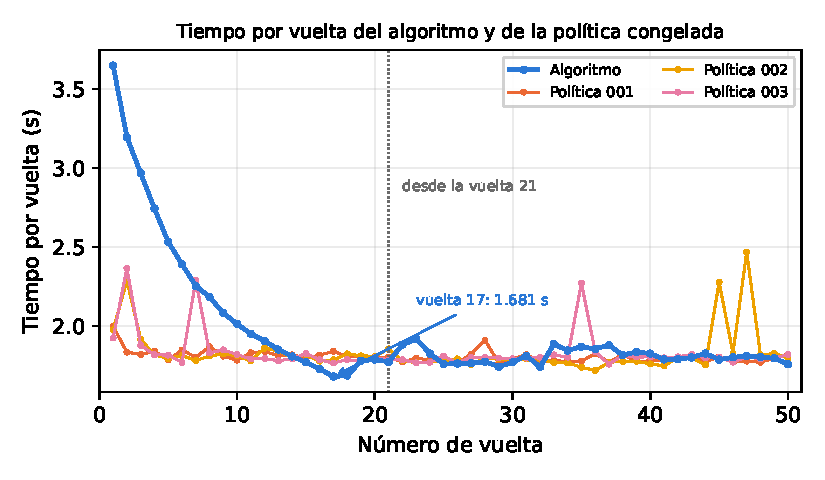
\includegraphics[trim={0 0 0 22},clip,width=\textwidth]{imaxes/PRUEBAS/POLITICA_OPTIMA/tiempos_politica.pdf}
  \caption{Tiempo por vuelta de las cuatro ejecuciones. Al algoritmo le cuesta catorce vueltas alcanzar el ritmo que la política ya lleva desde la primera}
  \label{fig:politica-tiempos}
\end{figure}

Si se descuentan esas vueltas de arranque la ventaja desaparece. La tabla~\ref{tab:politica-estable} recoge las mismas métricas a partir de la vuelta 21, que es cuando el tiempo del algoritmo deja de bajar, y las cuatro ejecuciones caben en 0,83~s sobre 30 vueltas, menos de tres centésimas por vuelta. Tampoco resulta la política más fiable, porque dos de las tres repeticiones derrapan bastante más que el algoritmo, con 82 y 96 muestras por encima del umbral frente a las 16 de la ejecución de referencia y con picos de 22,5 y 26,1~px que se traducen en vueltas sueltas de 2,468 y 2,366~s. Y eso que las tres se hicieron seguidas, en un cuarto de hora y sin tocar nada: el perfil congelado no puede echarse atrás cuando la pista cambia bajo él, mientras que el algoritmo baja la tensión de la zona en cuanto detecta el derrape.

\begin{table}[tbp]
  \centering
  \estilotabla[3]
  \caption{Las mismas métricas contando solo desde la vuelta 21, con el algoritmo ya estabilizado.}
  \label{tab:politica-estable}
  \begin{tabular}{lrrrrr}
    \toprule
    \rowcolor{ArqAzulClaro}
    Ejecución & Contrarreloj & Mejor & Mediana & Media & $\sigma$ \\
              \rowcolor{ArqAzulClaro} & (s) & (s) & (s) & (s) & (s) \\
    \midrule
    Política 001 & 53,85 & 1,766 & 1,783 & 1,795 & 0,028 \\
    Algoritmo    & 54,33 & 1,742 & 1,804 & 1,811 & 0,045 \\
    Política 003 & 54,43 & 1,760 & 1,803 & 1,814 & 0,087 \\
    Política 002 & 54,68 & 1,719 & 1,785 & 1,823 & 0,152 \\
    \bottomrule
  \end{tabular}
\end{table}

La conclusión es que aplicar una política fija sí permite empezar con buenos tiempos desde la primera vuelta, mientras que el algoritmo necesita unas cuantas iteraciones para llegar ahí, pero no da ninguna ventaja de ritmo y se paga con la adaptabilidad, ya que si el circuito cambia el algoritmo se adapta solo y la política hay que rehacerla. Guardarla tiene sentido para repetir carreras sobre un circuito que no se va a desmontar, y de hecho lo que esta prueba señala como mejorable del algoritmo no es su ritmo, que ya es el bueno, sino la rampa con la que arranca: partir de un perfil guardado o subir a escalones más grandes en las primeras vueltas le ahorraría los siete segundos que aquí pierde.

\section{Pruebas de red}
\label{sec:pruebas-red}

El objetivo de esta prueba es comprobar cuanto retardo añade la red al lazo de control y a partir de qué punto llega a notarse en la pista. Se hizo sobre el óvalo con una sola cámara, que es el trazado del que más datos se tienen y ser más sencillo de trabajar.

Todas las ejecuciones se hicieron con el coche azul, en el mismo carril, con la cámara sin mover y con la misma configuración: rango de PWM de 65 a 90 y umbral de derrape de 10~px. De cada escenario se hicieron tres repeticiones de 50 vueltas, 18 ejecuciones en total.

El retardo no se puede medir restando la marca de tiempo que la cámara pone en el mensaje menos el instante en que el controlador lo recibe, porque son dos relojes de dos máquinas distintas lo que puede ocasionar que haya desfase entre ellas. Por eso se añadió un nodo que manda a la cámara paquetes del tamaño de un mensaje de posición y cronometra lo que tardan en volver. Al ser un viaje de ida y vuelta las dos marcas las toma el mismo reloj y el desfase desaparece al restar, que es el motivo por el que el RFC~2681 define una métrica de ida y vuelta~\cite{rfc2681}. La cámara devuelve también lo que ha tardado ella en contestar, y ese tiempo se descuenta. De forma que el retardo podemos estimar como la mitad del tiempo que tardamos en hacer el viaje de ida y vuelta.

En los tres escenarios el nodo puente se ejecuta en la misma máquina que los controladores. Es una decisión de despliegue y no una limitación, esa máquina ya tiene que ser potente porque lleva un controlador por coche, y teniendo ese equipo lo razonable es enchufarle el Arduino y no añadir un salto de red entre decidir la tensión y aplicarla. La arquitectura permite separarlos, pero ese caso no se ha probado.

Los tres escenarios se diferencian solo en dónde corre el nodo cámara. En el primero, A1, los tres nodos están en el mismo ordenador y no hay red de por medio. En el segundo, A2, la cámara corre en la Raspberry Pi y conectado por cable al router al igual que el ordenador, y en el tercero, A3, la misma cámara conectaod por WIFI al router igual que el ordenador. Lo que viaja por ese enlace es la posición del coche, que es lo que el controlador necesita para aplicar el algoritmo.

La tabla~\ref{tab:red-rtt} recoge lo que mide el nodo de sondeo, el nodo que se creo y que envía mensajes para medir el tiempo de ida y vuelta. El peor escenario es el WiFi y aun así se queda en 7,27~ms de mediana, y en ninguno de los tres se perdió un solo paquete de los más de mil seiscientos que se enviaron. Que A1 no salga a cero, e incluso quede por encima del cable, puede ser algo no tan raro ya que esa máquina lleva encima además el nodo cámara, y pasar un mensaje entre dos procesos tampoco es gratis.

\begin{table}[tbp]
  \centering
  \estilotabla[3]
  \caption{Tiempo de ida y vuelta por escenario, con las tres repeticiones juntas.}
  \label{tab:red-rtt}
  \begin{tabular}{lrrrrr}
    \toprule
    \rowcolor{ArqAzulClaro}
    Escenario & Sondeos & Mediana & p95 & p99 & Máximo \\
              \rowcolor{ArqAzulClaro} & & (ms) & (ms) & (ms) & (ms) \\
    \midrule
    A1 (una máquina) & 1680 & 3,36 & 8,74 & 19,80 & 54,27 \\
    A2 (cable)       & 1720 & 2,42 & 10,00 & 12,54 & 16,92 \\
    A3 (WiFi)        & 1664 & 7,27 & 14,96 & 17,76 & 27,80 \\
    \bottomrule
  \end{tabular}
\end{table}

La figura~\ref{fig:red-cdf} enseña la medida completa. Las tres curvas suben de golpe y se plantan antes de los 20~ms. La del WiFi va desplazada unos milisegundos a la derecha de las otras dos, y esa es toda la diferencia entre las tres.

\begin{figure}[tbp]
  \centering
  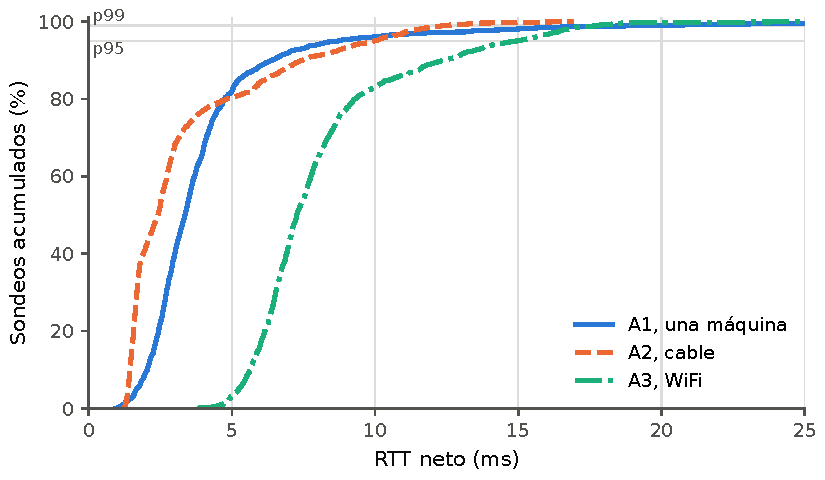
\includegraphics[width=\linewidth]{imaxes/PRUEBAS/RED/cdf_rtt.pdf}
  \caption{Distribución acumulada del tiempo de ida y vuelta. Fuera del eje queda un único sondeo de A1 de 54~ms.}
  \label{fig:red-cdf}
\end{figure}

Esos milisegundos hay que verlos al lado del resto del lazo, y eso es lo que hace la figura~\ref{fig:red-presupuesto}, que muestra como se reparte la latencia entre los tres pasos que van desde que se captura el fotograma hasta que el algoritmo devuelve el valor que hay que aplicar de tensión. El de la red es el más pequeño de los tres con diferencia, incluso por WiFi no llega a una quinta parte del total, que se queda en 22~ms. Y ese total cabe dentro de los 33~ms que pasan entre dos fotogramas.

\begin{figure}[tbp]
  \centering
  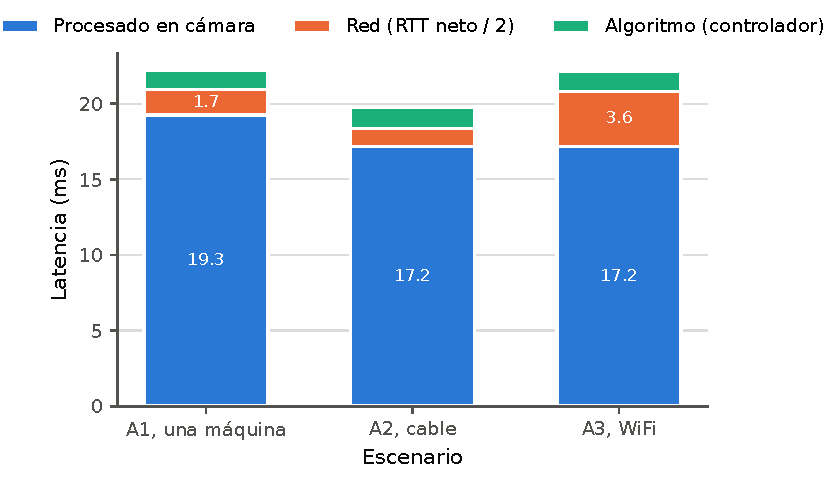
\includegraphics[width=\linewidth]{imaxes/PRUEBAS/RED/presupuesto_latencia.pdf}
  \caption{Reparto de la latencia del lazo entre sus tres pasos. El tramo de red es la mitad del tiempo de ida y vuelta.}
  \label{fig:red-presupuesto}
\end{figure}

Sobre la pista no se traduce en nada, y eso lo dice la tabla~\ref{tab:red-tiempos-a}. Los tres escenarios completan las 50 vueltas en un tiempo parecido y sus mejores vueltas se quedan en cuatro centésimas unas de otras, con el WiFi como el más rápido de los tres aun siendo el que más retardo tiene. Las tres repeticiones de A2 dieron 97,35, 100,63 y 104,51~s, así que dos ejecuciones del mismo escenario se separan más que los escenarios entre sí. Lo que se ve ahí es la variabilidad del coche y del circuito que ya describe la sección~\ref{sec:prueba_pwm_incremental}.

\begin{table}[tbp]
  \centering
  \estilotabla[3]
  \caption{Tiempos de las 50 vueltas por escenario.}
  \label{tab:red-tiempos-a}
  \begin{tabular}{lrrrrr}
    \toprule
    \rowcolor{ArqAzulClaro}
    Escenario & Contrarreloj & Mejor & Mediana & Media & $\sigma$ \\
              \rowcolor{ArqAzulClaro} & (s) & (s) & (s) & (s) & (s) \\
    \midrule
    A3 (WiFi)        & 97,91 & 1,725 & 1,819 & 1,958 & 0,285 \\
    A2 (cable)       & 100,83 & 1,716 & 1,808 & 2,017 & 0,552 \\
    A1 (una máquina) & 102,45 & 1,740 & 1,843 & 2,049 & 0,405 \\
    \bottomrule
  \end{tabular}
\end{table}

Que la red no se note cuando es buena no dice hasta dónde aguanta el control cuando deja de serlo. Para verlo se repitió el escenario del WiFi añadiendo retardo a mano con \texttt{tc netem}~\cite{netem}, una herramienta del \emph{kernel} de Linux que retiene los paquetes el tiempo que se le indique. La regla se pone en la Raspberry Pi con \texttt{sudo tc qdisc add dev wlan1 root netem delay 25ms}, se pasa de un punto al siguiente cambiando \texttt{add} por \texttt{change}, y al terminar se quita con ese mismo comando y \texttt{del}. Se probaron 25, 50 y 100~ms, con tres repeticiones cada uno. No se subió más porque con más de 100~ms entre dos máquinas de la misma sala el problema ya no es el control.

Como la regla está en la salida de la Raspberry Pi, el retardo lo sufre el sentido cámara~$\rightarrow$~PC, que es justamente por donde viajan las posiciones, y por eso aparece una sola vez en el tiempo de ida y vuelta de la tabla~\ref{tab:red-tiempos-b}. Con 100~ms cada posición que recibe el controlador dice dónde estaba el coche hace una décima de segundo. Con el retardo puesto aparecen además mensajes perdidos, trece de unos cinco mil, pero concentrados en dos repeticiones sueltas y sin relación con el retardo aplicado.

\begin{table}[tbp]
  \centering
  \estilotabla[3]
  \caption{Retardo medido y tiempos de las 50 vueltas según el retardo inyectado. El punto de 0~ms es A3 sin tocar.}
  \label{tab:red-tiempos-b}
  \begin{tabular}{lrrrrrr}
    \toprule
    \rowcolor{ArqAzulClaro}
    Retardo & Ida y vuelta & Contrarreloj & Mejor & Mediana & Media & $\sigma$ \\
            \rowcolor{ArqAzulClaro}
    inyectado & (ms) & (s) & (s) & (s) & (s) & (s) \\
    \midrule
    0 ms   & 7,27 & 97,91 & 1,725 & 1,819 & 1,958 & 0,285 \\
    25 ms  & 33,21 & 100,98 & 1,750 & 1,870 & 2,020 & 0,322 \\
    50 ms  & 58,48 & 99,69 & 1,730 & 1,857 & 1,994 & 0,307 \\
    100 ms & 108,35 & 105,41 & 1,735 & 1,889 & 2,108 & 0,427 \\
    \bottomrule
  \end{tabular}
\end{table}

El coche completa sus 50 vueltas en los cuatro casos y la mejor vuelta no empeora en ninguno. Con 25 y 50~ms los tiempos no se distinguen del punto de partida. Con 100~ms sí aparece algo: las tres repeticiones de ese punto dieron 103,46, 105,16 y 107,62~s, todas por encima de cualquiera de las tres sin retardo, y la vuelta mediana sube de 1,819 a 1,889~s, es una subida pequeña pero relevante.

La conclusión es que la red no es lo que limita el control. Por cable o por WiFi añade unos pocos milisegundos, muy por debajo de lo que tarda la propia cámara en procesar el fotograma, y el sistema se comporta igual que con todo junto en una máquina. Hay que inyectar 100~ms, más de diez veces el peor retardo medido aquí, para que empiece a notarse algo, y ni siquiera entonces el coche pierde el control. Encaja con lo observado durante el resto del trabajo, ya que buena parte de las pruebas con dos cámaras se hicieron por WiFi sin que se notara ninguna diferencia.

\section{Pruebas en Circuitos Grandes}
\label{sec:pruebas-circuitos-grande}

Aparte de los resultados obtenidos en la realización de las pruebas de red, también hicimos dos circuitos un poco grandes para demostrar que la arquitectura es completamente funcional en circunstancias distribuidas con multiples camaras como también estaba pensado. Vamos a tener dos circuitos donde vamos a ver como se comporta el coche si somos capaces de controlador y ver lo qeu pasa. Para está prueab vamos va tener 2 rasberry pi 5 para controlar cada una como nodo camara y después en el ordenador vamos a tener un controlador y el nodo puente que permite controlar el arduino. 

\section{Prueba nodo visualización y multiples coches}
\label{sec:prueba-nodo-visualizacion-multiples-coches}

Esta es una pequeña prueba para ver como se comporta la arquitectura con varios coches y como funciona además el nodo de visualización que tenemos creado para controlarlo 
